\documentclass[12pt,a4paper]{report}

% Retain the project-report structure while applying the dissertation module's
% explicit 12-point and A4 formatting requirements.
\usepackage[margin=25mm,headheight=14pt]{geometry}
\usepackage{setspace}
\usepackage{amsmath,amssymb}
\usepackage{array}
\usepackage{booktabs}
\usepackage{enumitem}
\usepackage{graphicx}
\usepackage{placeins}
\usepackage{longtable}
\usepackage{microtype}
\usepackage[numbers,sort&compress]{natbib}
\usepackage{tabularx}
\usepackage{tikz}
\usetikzlibrary{arrows.meta}
\usepackage{pgfplots}
\pgfplotsset{compat=1.18}
\usepackage{xcolor}
\usepackage[hidelinks]{hyperref}
\usepackage[capitalise,noabbrev]{cleveref}

\definecolor{sentineldark}{HTML}{17202A}
\definecolor{sentinelamber}{HTML}{D97706}
\definecolor{sentinelred}{HTML}{B42318}
\definecolor{sentinelblue}{HTML}{2563EB}
\definecolor{sentinelgrey}{HTML}{667085}

\hypersetup{
  pdftitle={Sentinel: Independent Runtime Enforcement for Browser Agents},
  pdfauthor={Hector Gittos},
  pdfsubject={MSc Information Security dissertation},
  pdfkeywords={browser agents, prompt injection, runtime enforcement, reference monitor, human in the loop}
}

\graphicspath{{./}}
\setlength{\emergencystretch}{2em}
\Urlmuskip=0mu plus 1mu
\setlength{\parindent}{1.5em}
\setlength{\parskip}{0pt}
\setlist{nosep}
\renewcommand{\arraystretch}{1.15}
\newcolumntype{L}[1]{>{\raggedright\arraybackslash}p{#1}}
\newcolumntype{Y}{>{\raggedright\arraybackslash}X}

\newcommand{\systemname}{\textsc{Sentinel}}
\newcommand{\studentname}{Hector Gittos}
\newcommand{\degreeprogramme}{MSc Information Security}
\newcommand{\submissiondate}{September 2026}
\newcommand{\supervisorname}{Arthur}
\newcommand{\rqone}{To what extent can an independent runtime-enforcement layer reduce prompt-injection-driven browser-agent violations while retaining useful task performance?}

\begin{document}
% Use explicit one-and-a-half spacing as required by the dissertation module.
\onehalfspacing

\hypersetup{pageanchor=false}
\begin{titlepage}
  \centering
  
\includegraphics[width=0.28\textwidth]{ucl_logo.png}\par
  \vspace{1.5cm}
  {\Huge\bfseries Sentinel: Independent Runtime Enforcement for Browser
  Agents\par}
  \vfill
  {\Large \studentname\par}
  \vspace{0.6cm}
  {\large \degreeprogramme\par}
  \vspace{0.6cm}
  {\large Submission date: \submissiondate\par}
  \vspace{0.35cm}
  {\large Supervisor: \supervisorname\par}
  \vfill
  \begin{minipage}{0.88\textwidth}
    \small
    \textbf{Declaration.}
    This report is submitted in partial fulfilment of the requirements for the
    \degreeprogramme\ at University College London. It is substantially the
    result of my own work except where explicitly indicated in the text.

    \medskip
    \textbf{Distribution statement.}
    The report may be freely copied and distributed provided the source is
    explicitly acknowledged.
  \end{minipage}
\end{titlepage}

\pagenumbering{roman}
\hypersetup{pageanchor=true}

\chapter*{Abstract}
\addcontentsline{toc}{chapter}{Abstract}
\begin{singlespace}

Browser agents turn model outputs into consequential actions, yet the pages
they must interpret may also contain instructions supplied by an attacker.
This creates an authority problem: the acting model sees untrusted content
while deciding whether that content should influence privileged effects. This
dissertation presents \systemname, an independent enforcement layer between a
browser agent and its executor. \systemname\ governs the exact observation sent
to the model, evaluates proposed actions immediately before execution, and
transfers control when policy requires human authority. It combines
attributable observation sanitisation and re-detection, origin-scoped taint,
deterministic policy and data-flow rules, narrow approval, direct human steps
for protected input, and privacy-preserving audit through a Chrome extension.

The evaluation connects controlled mechanism evidence to browser-native
execution. Across paired AgentDojo comparisons with 629 attacked tasks per
condition, enforcement changed native attacker success from 206 to 0 cases for
Qwen 3.5 4B, from 131 to 1 for 9B, and from 203 to 0 for 27B, while utility
increased in all three enforce conditions. The principal WASP study repeats 84
browser tasks across three seeds under off, policy-only, and full conditions
($n=252$ per condition). From off to full, action-audited terminal attacker
success changed from 17/252 to 0/252 and attacker-directed execution from
42/252 to 0/252. Legitimate-task completion changed from 154/252 to 149/252,
while secure utility rose from 138/252 to 149/252. Without sanitisation,
enforcement still left attacker-directed execution in 15/252 episodes; the full
condition produced no attacker-directed proposal at the same aggregate utility
and recorded 740 confirmed sanitisation removals.

In these experiments, independently governing observations and actions sharply
reduced successful attacks and attacker-serving execution while retaining most
useful task completion. The result does not establish a universal defence. It
shows something narrower and practically important: a browser agent can still
plan useful work when another component decides which privileged effects may
occur.
\end{singlespace}

\begingroup
\small
\tableofcontents
\endgroup
\listoffigures
\listoftables
\clearpage

\pagenumbering{arabic}

\chapter{Introduction}
\label{chap:introduction}

\section{Motivation}

Large language models increasingly operate as agents: they observe an
environment, choose tools, inspect the result, and continue until a task is
complete. Browser agents apply this loop to navigation, form entry, file
handling, and web applications in which a model output can become an external
side effect. This capability is useful precisely because web tasks are rarely
one-shot questions: benchmarks such as WebArena require agents to carry state
across several dependent interactions~\cite{zhou2024webarena}.

The same loop creates a security problem. Web observations mix application
content, user-generated data, embedded resources, and text controlled by an
attacker. An indirect prompt injection places instructions in that data so the
agent encounters them while pursuing a legitimate goal~\cite{greshake2023indirect}.
The attack exploits an authority ambiguity rather than a malformed API call:
the model is expected to understand novel page content, yet must also decide
whether that content is entitled to redirect its behaviour. Once the model can
invoke privileged tools, a successful redirection can change remote state or
disclose information instead of merely producing incorrect prose.
Prompt reminders, delimiters, and detectors can reduce exposure, but they
leave the acting model responsible for respecting the distinction between the
operator's goal and hostile data. Classical protection principles suggest a
different allocation of responsibility. Complete mediation places a check at
each privileged use, while least privilege limits which component may perform
the effect~\cite{saltzer1975protection}. For an agent, the model can remain a
flexible planner without being the final authority for its proposed actions.
An independent runtime can enforce deterministic constraints, control data
flows, request narrowly scoped authority, and record the outcome.

\section{Research question and thesis}

The research question is:

\begin{quote}
\textbf{RQ.} \rqone
\end{quote}

Security and utility are evaluated together. A system that blocks every action
can suppress attacks while destroying the purpose of an agent; conversely,
high task completion is not useful if trajectories also achieve attacker
goals. The dissertation therefore measures native user-task success, native
attacker success, their joint outcome, and whether attacker-directed actions
reach the executor.

The thesis is that \emph{independent runtime enforcement can reduce evaluated
policy violations while preserving useful autonomy under the tested
conditions}. Independence means that an allow, block, approval, or takeover
outcome is determined outside the acting model. The claim is tied to defined
tool and browser benchmarks rather than to prompt injection in general.

\section{Approach}

This dissertation presents \systemname, a local research prototype positioned
between a BrowserUse agent and its privileged executor. It governs the agent
loop at two points. Before inference, an observation guard identifies
untrusted browser, extraction, and tool-result regions; detects configured
prompt-injection signals; removes attributable regions; and re-detects the
exact reconstructed model input. Before execution, an action guard rebuilds
live browser context, classifies capabilities and sensitive data, propagates
origin-scoped taint, and invokes one policy engine. The executor is reached
only after that decision.

Automatic enforcement is combined with selective human authority. Hard policy
and protected data flows remain non-overridable. A permissible but
consequential action can receive narrow, expiring approval and is evaluated
again against live state before execution. Recognised credentials, one-time
codes, payment data, and other protected values trigger direct takeover so the
operator performs the step instead of authorising the agent to type the value.
If a suspicious current-page observation cannot be sanitised and verified, it
is withheld and the operator may inspect the page before Sentinel captures a
fresh observation. A Chrome extension presents these states and the redacted
decision history; the server remains the source of authority.

Evaluation proceeds in two stages. AgentDojo supplies controlled tool-agent
tasks with native user and attacker oracles across four application domains
~\cite{debenedetti2024agentdojo}. WASP then exercises a BrowserUse agent over
mutable GitLab and Reddit environments, adding observation construction,
navigation, and browser re-planning~\cite{evtimov2025wasp}. The primary browser
result is a matched Qwen 3.5 27B off/enforce comparison. A provenance-separated
9B development sequence is retained because it explains why warning-only
enforcement and incomplete sanitisation were replaced by post-verified
removal.

\section{Contributions}
\label{sec:contributions}

The dissertation makes three contributions.

\begin{enumerate}
  \item \textbf{Executor-side enforcement for a dynamic browser-agent loop.}
  Sentinel interposes on model input and every model-proposed privileged action
  entering the governed executor. Live context, central policy evaluation,
  fail-closed outcomes, and paired attempted/terminal audit separate a model's
  proposal from authority to act without changing the underlying model.

  \item \textbf{Post-verified observation governance with selective
  authority.} Detection is connected to attributable sanitisation,
  reconstruction, and clean re-detection. Origin-scoped taint and action policy
  remain as backstops. Approval, direct takeover, and unresolved-observation
  incidents provide distinct server-owned paths for decisions that cannot be
  resolved as an automatic allow or block.

  \item \textbf{A two-environment security--utility evaluation.} Across 629
  attacked AgentDojo tasks per condition and model, enforcement reduced native
  attacker success from 206 to 0 cases for Qwen 3.5 4B, from 131 to 1 for 9B,
  and from 203 to 0 for 27B while utility increased in each row. In the matched
  27B WASP comparison, attacker success changed from 5/84 to 0/84 and
  attacker-directed execution from 17/84 to 0/84, while utility changed from
  47/84 to 46/84. Reporting intermediate execution together with utility avoids
  treating either inactivity or baseline model failure as security.
\end{enumerate}

Sentinel does not claim BrowserUse, AgentDojo, WASP, or Qwen as original work.
Its original contribution is the architecture that composes observation
governance, executor-side policy, selective authority, and paired audit around
a dynamic browser agent, together with the implementation and evaluation of
that composition.

\section{Dissertation structure}

\Cref{chap:background} establishes the prompt-injection and system-security
context. \Cref{chap:threat-model} defines the authority boundary and security
requirements. \Cref{chap:design} presents the implementation and operator
control plane. \Cref{chap:methodology,chap:results} define and report the
evaluation, and \cref{chap:discussion,chap:conclusion} interpret the evidence,
scope its validity, and state the resulting contribution.

\clearpage
\chapter{Background and related work}
\label{chap:background}

\section{Browser agents and indirect prompt injection}

An LLM agent places a generative model in a feedback loop of goals,
observations, decisions, tool calls, and results. ReAct made this
reasoning--action interleaving explicit, while Toolformer examined how models
can learn to invoke tools~\cite{yao2023react,schick2023toolformer}. Browser
agents bring the same loop into environments composed of URLs, structured page
representations, interactive elements, and code-capable actions. WebArena and
WorkArena evaluate such agents in executable environments with task-specific
evaluators, including state and answer checks
~\cite{zhou2024webarena,drouin2024workarena}. Together, these benchmarks
highlight two properties relevant here: success is a validated task outcome,
not merely a plausible response, and the agent's observations contain data
outside the operator's control.

This exposure creates a security problem because instructions and data share
the same model context. Direct prompt-injection attacks alter the user's
prompt; indirect attacks instead arrive through retrieved content that the
application expected to treat as data.
Greshake et al. demonstrated indirect prompt-injection attacks in synthetic
LLM-integrated applications and through local web content, including data
exfiltration and worm-like propagation~\cite{greshake2023indirect}. In a
browser setting, an attacker can place equivalent instructions in a page,
user-generated record, link label, or stored result, where the agent encounters
them while acting with the user's delegated authority. For example, injected
issue content can divert an agent asked to comment on an issue towards account
settings, with the attacker goal of making the benchmark user's profile public
~\cite{evtimov2025wasp}. The page supplies the hostile instruction, but the
resulting navigation occurs within the benchmark user's authenticated sandbox
session.

Indirect prompt injection therefore differs from conventional parser
injection. A browser agent is deliberately expected to interpret previously
unseen prose, so a fixed grammar cannot by itself establish which source has
authority. Delimiters can mark the distinction between trusted instructions
and untrusted input, but page text can imitate them, leaving the model to decide
which instruction deserves authority. Formal analyses and benchmark studies
reinforce this point: models do not reliably distinguish the instructions they
should follow from external content they should treat as data
~\cite{liu2024formalizing,yi2025bipia}.

Nor is the threat confined to the current page. Retrieved content can influence
subsequent model responses and API calls, while persistent memory can
reintroduce hostile content in later sessions~\cite{greshake2023indirect}.
Multimodal agents add a further channel: image-hijack work shows that specially
optimised adversarial images can carry the behavioural effect of a chosen text
prompt and redirect a vision-language model's behaviour
~\cite{bailey2024imagehijacks}. A filter over the Document Object Model (DOM),
the browser's structured representation of a page, cannot remove content
rendered only in pixels. Visual observations therefore form a distinct threat
surface that requires its own controls; text sanitisation does not automatically
cover it.

\subsection{What an agent-security evaluation must measure}

These threat surfaces also make the unit of evaluation important. A detector
labels a piece of text; an action monitor labels a proposed or executed effect;
and an end-to-end oracle checks whether the user or attacker changed the
environment as intended. High detector recall can still coexist with a
compromised trajectory if the model is merely warned or a dangerous effect
bypasses the monitored channel. Conversely, low terminal attack success can
describe an agent that was diverted but lacked the capability or remaining
steps to complete the attack.

AgentDojo operationalises this distinction by pairing realistic user tasks with
attacker goals in executable banking, messaging, travel, and workspace
environments~\cite{debenedetti2024agentdojo}. Its native oracles score both
goals through task-specific checks that may inspect environment state and model
output. WASP makes a related distinction for browser agents, using an LLM judge
to assess whether a trajectory has been diverted before the terminal attacker
goal is achieved~\cite{evtimov2025wasp}. The benchmarks are therefore
complementary: AgentDojo provides controlled tool-agent environments, whereas
WASP adds browser-native observations, navigation, and re-planning. Their
absolute rates cannot be pooled, however, because their tasks, action spaces,
and oracles differ. ST-WebAgentBench broadens the picture further by studying
policy compliance through Completion Under Policy and Risk Ratio
~\cite{levy2026stwebagentbench}. These measures must be read together because
detection, risky execution, policy compliance, and final-state success reveal
different parts of system behaviour.

Accordingly, this dissertation treats security and utility as a joint outcome.
It reports native user completion, native attacker success, useful-and-secure
completion, attacker-directed attempts and executions, and recorded
enforcement events alongside trajectory outcomes, while separating scripted
controls from actual human intervention. This combination guards against two
misleading conclusions: calling an inactive agent secure, or calling a capable
but compromised agent useful.

\section{Defence design space}

\subsection{Model-facing defences}

One family of defences tries to help the planner recognise which content
deserves instructional authority. BIPIA evaluates reminders, boundary
awareness, in-context examples, and training across indirect-injection tasks
~\cite{yi2025bipia}. Spotlighting takes a complementary approach, using
delimiting, datamarking, or encoding to keep the distinction between trusted
instructions and untrusted input salient to the model
~\cite{hines2024spotlighting}.

Other approaches try to make this separation part of model behaviour. StruQ
uses structured instruction tuning to distinguish prompt and data channels
~\cite{chen2025struq}, while SecAlign uses preference optimisation to favour
responses that follow the legitimate instruction over the injection
~\cite{chen2025secalign}. Both report greater resistance to the evaluated
attacks with limited utility loss in their respective settings. More
specifically, on its principal AlpacaFarm evaluation, SecAlign reports 0\%
attack success for the evaluated optimisation-free attacks and rates mainly
below 10\% for stronger optimisation-based attacks, with utility similar to its
non-preference-optimised counterparts. A separate out-of-distribution SEP
Ignore evaluation reports 11.0\%, 3.6\%, and 6.5\% attack success when the
injection appears at the start, middle, and end of the input. These findings
remain bound to the paper's models, tasks, and attacks. A later diagnostic shows
why attack rejection and benign utility must be read together. Across three
reasoning benchmarks, benign suffix-task rejection in the evaluated fine-tuned
defences rose from below 10\% to as high as 90\%. The authors link these
failures to position, trigger-token, and topic correlations, suggesting that
trained defences can rely on narrow surface cues without reliably identifying
malicious intent~\cite{li2026surfaceheuristics}.

Model-facing checks can also operate during inference. Task Shield asks whether
each instruction and proposed tool call contributes to the user's stated goal
~\cite{jia2025taskshield}. Under the one-trial-per-task Important
Instructions attack condition on AgentDojo with GPT-4o, its authors report
2.07\% attack success and 69.79\% utility under attack. MELON instead reruns
the agent trajectory with the user prompt masked and treats similarity between
the original and counterfactual tool calls as evidence of hijacking. The paper
notes that response-based attacks without tool calls can evade this comparison
~\cite{zhu2025melon}. Although their mechanisms differ, both examine whether
planned behaviour remains dependent on the authorised task and report
AgentDojo trade-offs within their own configurations. Sentinel additionally
tests transfer through WASP's browser-native loop. Even within AgentDojo,
however, differences in models, attack construction, scaffolds, defence
mechanisms, and metric definitions make headline rates contextual; they do not
provide a controlled ranking against Sentinel.

Detection offers another inspectable intervention before processed content
reaches the downstream LLM. Detect-and-Remove separates document-level attack
identification from sentence-level removal or generative extraction followed
by longest-common-substring removal~\cite{chen2025detectremove}. The approach
therefore depends on detecting the attack and identifying what can be removed
without losing information needed to complete the task. Distribution shift
adds a broader challenge: no fixed collection of examples can cover every
wording, encoding, page context, or adaptive strategy. Indeed, white-box
optimisation against specific defences has outperformed non-adaptive attacks in
the evaluated settings~\cite{zhan2025adaptive}. These limitations motivate
Sentinel's layered use of detection: it governs observations while policy is
applied independently before execution. Model-facing guidance is thus backed
by external checks on what the agent observes and can do, keeping execution
authority outside the model.

\subsection{System-level authority}

Where model-facing defences influence planning, system-level work moves selected
security and execution decisions outside unconstrained model reasoning. Some
designs nevertheless retain LLM components within the wider control
architecture. CaMeL, for example, extracts control and data flow from a trusted
query, confines untrusted data to constrained processing, and enforces
capabilities at tool calls~\cite{debenedetti2025camel}. Fides instead applies
information-flow control: confidentiality and integrity labels propagate
through planning, deterministic policies govern tool effects, and information
can be selectively hidden from the planner~\cite{costa2025fides}. Progent
represents privilege as symbolic rules over tool names and arguments, checks
every tool call deterministically, applies privilege narrowing automatically,
and can require approval before an expansion. Its main experiments use
Auto-Approve, so they do not measure human-reviewed expansion
~\cite{shi2025progent}. Building on Fides, PRUDENTIA makes planning policy-aware
and evaluates autonomy through task completion at intervention budgets and
trace-derived oversight load under assumed approval
~\cite{kolluri2026prudentia}.

Other systems place trust in different abstractions. AgentSpec provides a
lightweight language of triggers, predicates, and runtime enforcement actions
~\cite{wang2026agentspec}. DRIFT derives a minimal function trajectory and
parameter checklist from the trusted query, validates deviations, and masks
conflicting instructions before they persist in memory~\cite{li2025drift}.
IPIGuard plans an initial tool-dependency graph before exposure to external data
and constrains later execution to its traversal, while allowing read-only query
nodes to be added during execution~\cite{an2025ipiguard}. VIGIL takes a
different route: it permits speculative reasoning over the tool stream, then
verifies a proposed effect against the trusted intent before commitment
~\cite{lin2026vigil}. AttriGuard instead tests whether a proposed tool call
survives teacher-forced shadow replay under control-attenuated external
observations~\cite{he2026attriguard}. Their reported attack-success rates are
not directly comparable, since each system changes a different part of the
agent stack and is evaluated under different policies, models, and tasks.
Moreover, each assurance remains conditional on the system's trusted
abstraction and expressible policy. \Cref{tab:system-comparison} therefore asks
the more durable architectural question: what does each system trust, and where
is that trust enforced?

\begin{table}[!t]
\centering
\caption{Representative system-level approaches.}
\label{tab:system-comparison}
\footnotesize
\renewcommand{\arraystretch}{1.08}
\setlength{\tabcolsep}{3.5pt}
\begin{tabularx}{\textwidth}{@{}L{0.16\textwidth}L{0.22\textwidth}L{0.22\textwidth}Y@{}}
\toprule
System & Trusted abstraction & Enforcement boundary & Evidence and assurance \\
\midrule
CaMeL~\cite{debenedetti2025camel} &
Trusted-query program and capabilities &
Structured flow and tool calls &
By-design guarantees for supported flows; AgentDojo. \\
\addlinespace[2.25pt]

Fides\newline\cite{costa2025fides} &
Security labels and flow policy &
Planner exposure and tools &
Formal IFC; AgentDojo. \\
\addlinespace[2.25pt]

Progent\newline\cite{shi2025progent} &
Generated symbolic tool and argument privileges &
Every call and privilege expansion &
Deterministic confinement; AgentDojo and ASB. \\
\addlinespace[2.25pt]

PRUDENTIA\newline\cite{kolluri2026prudentia} &
Fides labels and policy-aware planning &
Planning, exposure, endorsement, and tools &
Inherited deterministic IFC; AgentDojo and WASP under assumed approval. \\
\addlinespace[2.25pt]

AgentSpec~\cite{wang2026agentspec} &
Trigger--predicate--enforcement rules &
Configured runtime events &
Empirical evaluation in code, embodied, and driving domains. \\
\addlinespace[2.25pt]

AttriGuard~\cite{he2026attriguard} &
Survival under control-attenuated observations &
Shadow replay before tool execution &
Static: four LLMs and two benchmarks; adaptive: two backbones on a 61-case
AgentDojo subset. \\
\addlinespace[2.25pt]

\systemname &
Trusted request, policy, live context, and narrow server-owned authority &
Wrapped model-input regions and pre-execution actions &
Contract tests; AgentDojo and matched WASP outcomes. \\
\bottomrule
\end{tabularx}
\end{table}

The table shows differences in coverage, not a universal ordering. Progent and
AttriGuard mediate the action boundary; Sentinel also
governs wrapped planner observations. Sentinel nevertheless preserves
open-ended replanning, so policy can reject prohibited effects but cannot prove
that an allowed click advances the operator's goal. Its claim is therefore
limited to the evaluated observation, action, and authority boundaries, not
universal superiority.

\section{Protection principles for agent runtimes}

These system-level approaches connect to established protection principles.
The reference-monitor concept requires a mechanism to be invoked on every
protected operation, isolated from the subject it constrains, and small enough
to analyse~\cite{anderson1972computersecurity}. Complete mediation, fail-safe
defaults, and least privilege provide corresponding design tests
~\cite{saltzer1975protection}. A language model is a poor monitor for its own
effects because hostile input can influence its internal state. A
wrapper at the executor can instead satisfy the structural requirement that
every action in its governed tool path crosses one decision point, even though
natural-language risk classification remains empirical.

Information-flow control provides a complementary perspective by asking where
data originated and which sinks it may reach. Denning's lattice model
formalised label-constrained flow~\cite{denning1976lattice}. Browser-agent
values are less structured, however: page content becomes model context, and a
click can disclose information without an explicit network API. At each action
assessment, Sentinel therefore derives a bounded dynamic model. Wrapped browser
observations carry untrusted provenance, detections add injection taint,
recognised values add sensitive categories, and actions expose capabilities
such as navigation, page write, file access, and code execution. These labels
give the policy engine concrete source--sink facts to enforce at execution
time. They remain operational controls, however, and do not prove that every
information flow is isolated.

Finally, runtime enforcement needs a precise authority protocol. Effective
human-in-the-loop security depends on communication, processing, application,
and resulting behaviour~\cite{cranor2008humanloop}; automation research
likewise distinguishes information acquisition, information analysis, decision
and action selection, and action implementation
~\cite{parasuraman2000automation}. Drawing on this separation, Sentinel maps
hard refusal, narrow approval, takeover, and observation review to distinct
server outcomes. This structure prevents a generic confirmation from weakening
a hard rule. Whether the interface helps people make sound choices remains a
separate human-subject question, particularly because warning design affects
attention and response~\cite{sunshine2009cryingwolf,akhawe2013warningland}.

\section{Research gap}

Taken together, prior work spans learned separation, detection, structured
control, information flow, and runtime rules. The question motivating this
dissertation is therefore not whether one defence can eliminate prompt
injection. It is whether an independent layer placed between a browser agent
and its privileged executor can govern both the observations that shape
planning and the actions that produce effects, while retaining useful
replanning and reducing attacker-serving execution. Sentinel addresses this
narrower gap by combining model-input
mediation with pre-execution policy and server-owned authority. Its evidence is
deliberately divided: AgentDojo examines the enforcement mechanism under
controlled tool-agent conditions; WASP tests transfer to a browser-native
observation and navigation loop; and contract tests with deterministic
walkthroughs provide implementation evidence for the operator-authority
workflow. Together, these strands ask whether evaluated policy violations can
be reduced without eliminating useful autonomy, rather than claiming a general
solution to prompt injection or evidence about human behaviour.

\clearpage
\chapter{Threat model and security requirements}
\label{chap:threat-model}

\section{System model}

The operator supplies a trusted task goal \(G\). At agent step \(t\), the
browser produces an observation \(O_t\), the model and scaffold produce a
proposed action \(a_t\), and the privileged executor may update environment
state \(S_t\):

\[
  O_t = \mathsf{observe}(S_t), \qquad
  a_t = \mathsf{agent}(G,O_{\leq t},A_{<t}), \qquad
  S_{t+1} = \mathsf{execute}(S_t,a_t).
\]

In an ungoverned loop, the last transition follows directly from the model's
proposal. \systemname\ inserts an observation transformation
\(\mathsf{guard}_{O}\) and an action decision
\(\mathsf{guard}_{A}\):

\[
  \widehat{O}_t = \mathsf{guard}_{O}(O_t,P,C_t), \qquad
  d_t = \mathsf{guard}_{A}(a_t,S_t,P,C_t),
\]

where \(P\) is live policy and \(C_t\) is run-local governance state, including
taint, approvals, budgets, and cancellation. The executor is called only when
\(d_t\) yields \emph{allow} or a still-valid approved scope. Block, timeout,
cancellation, unavailable required context, and unresolved authority do not
execute \(a_t\).

This model separates \emph{proposal} from \emph{authority}. The model can
propose any syntactically valid tool call, including one influenced by
malicious content. The proposal has no effect until a component outside the
model evaluates it. The separation is the primary architectural security
property; the quality of individual detector and risk rules is a secondary,
empirical property.

\section{Actors, assets, and trust boundaries}

\begin{table}[htbp]
\centering
\caption{Actors and trust assumptions.}
\label{tab:trust-boundaries}
\small
\begin{tabularx}{\textwidth}{@{}L{0.25\textwidth}L{0.18\textwidth}Y@{}}
\toprule
Component or actor & Trust & Rationale \\
\midrule
Operator request and live steering & Trusted authority &
Defines the task and may provide new instructions, but cannot override a
configured hard block merely by approving a pending action. \\

Local policy and \systemname\ middleware & Trusted computing base &
Defines the allowed authority and mediates wrapped model inputs and
model-proposed privileged tool actions at the governed boundary. It does not
mediate direct human page interaction or browser effects outside those
channels. \\

Browser-agent model and scaffold & Untrusted decision maker &
May hallucinate, follow injected content, retry denials, or produce malformed
actions. \\

DOM, accessibility text, title, URL-carried content, extracted text, downloads,
and tool results & Untrusted data &
May contain first-party, third-party, user-generated, or attacker-controlled
content, including stored attacks. \\

Screenshot pixels & Excluded from ordinary model and operator-telemetry paths &
DOM sanitisation cannot clean text rendered into pixels. Optional local trace
retention does not make a frame trusted. \\

Browser and tool implementation & Privileged executor &
Performs effects after mediation and therefore remains inside the trusted
computing base. \\

Extension side panel & Operator interface, not an authority source &
Displays redacted decisions and submits responses that the server validates;
it cannot mint broader consent locally. \\

Trace consumers & Honest but curious &
May inspect records but should not receive raw secrets, injected payloads,
screenshots, or model rationale by default. \\

Other same-user processes & Outside the accepted boundary &
Loopback binding is accepted for this local research prototype; it does not
isolate the service from a compromised process with the same operating-system
account. \\
\bottomrule
\end{tabularx}
\end{table}

Protected assets include the operator's task authority, authenticated browser
session, private or security-sensitive data, local files available for upload,
integrity of remote state, consent decisions, and the confidentiality of audit
records. Availability is a secondary asset: a defence that blocks every task
is not useful, but fail-closed denial is preferred to an unauthorised side
effect when required security context is missing.

\section{Adversary}

The primary adversary controls content that the agent may encounter during a
legitimate task. This includes a page or part of a page, a user-generated
record, a link label, a tool result, or content later returned by extraction.
The adversary knows the general agent design and may write natural-language
instructions intended to:

\begin{itemize}
  \item replace or extend the operator's goal;
  \item impersonate system, developer, tool, or user authority;
  \item demand secrecy or suppression of warnings;
  \item request navigation, disclosure, code execution, file access, or a
  consequential same-origin action;
  \item persist influence through history or a second model call; or
  \item exploit ambiguities in page structure and target semantics.
\end{itemize}

The attacker need not compromise the model provider, \systemname\ process,
browser binary, operating system, or local policy file. Those stronger
attackers are out of scope. The benchmark adversary is also bounded by each
suite's instantiated attack goal and environment; the evaluation does not
claim coverage of every adaptive or obfuscated payload.

\section{Security objectives}
\label{sec:security-objectives}

The design is governed by eight objectives.

\begin{enumerate}[label=\textbf{O\arabic*:},leftmargin=16mm]
  \item \textbf{Complete action mediation.} Every model-proposed privileged
  tool action entering \texttt{GovernedTools} is evaluated immediately before
  execution. There is no model-accessible parallel path to the wrapped tool
  through the implemented agent scaffold.

  \item \textbf{Complete terminal audit.} Every such governed tool attempt has
  exactly one privacy-preserving attempted event and one terminal event,
  including blocks, denials, timeouts, exceptions, and cancellation.

  \item \textbf{Source does not imply authority.} Browser, file, extraction,
  and tool-result content remains untrusted even when it is necessary for the
  task or originates on the current first-party domain.

  \item \textbf{Controlled sensitive-data flow.} Recognised sensitive values
  cannot enter an untrusted sink solely because a page or the model requested
  it. In enforce mode, credentials, one-time codes, access tokens, payment
  values, private keys, and protected placeholders are completed by the human
  directly, not approved for agent entry.

  \item \textbf{Fail-safe authority.} Consent is explicit, narrow, expiring,
  run-local, and non-transferable. Silence, timeout, malformed responses,
  shutdown, and a stop race do not execute the pending action.

  \item \textbf{Observation post-condition.} Sanitisation counts as successful
  only if at least one attributable untrusted region changed and re-detection
  over the resulting model input is clear. A known residual or unattributable
  current browser observation is withheld before the model call.

  \item \textbf{Monitoring confidentiality.} Dedicated enforcement fields
  retain redacted summaries, finding metadata, and run-keyed digests, not raw
  detector payloads, recognised secrets, or unredacted parameters. Model
  metadata omits HTTP(S) queries and fragments; telemetry may retain benign ones
  after sensitive-value masking. Both omit non-web suffixes. Recursive
  redaction covers general events and history. Arbitrary model echoes and the
  local process log are outside this invariant.

  \item \textbf{Utility-aware enforcement.} Read-only inspection remains
  available where policy permits it, and ambiguous risk is not converted into
  a blanket block. The evaluation must report legitimate utility beside
  security outcomes.
\end{enumerate}

Objectives O1--O7 are implementation invariants within the channel scopes
defined above. O8 is a design and evaluation criterion rather than a universal
guarantee: no runtime can ensure task completion for an arbitrary model,
website, and policy.

\section{Taint and capability model}

\systemname\ assigns labels to sources and action parameters. A web observation
introduces \texttt{untrusted\_web}. A positive detector finding adds
\texttt{prompt\_injection\_suspected} and is retained per origin so that a
later clean viewport does not erase possible influence on model history.
Recognised values add categories such as \texttt{sensitive:credential},
\texttt{sensitive:one\_time\_code}, \texttt{sensitive:access\_token},
\texttt{sensitive:payment\_data}, or \texttt{sensitive:private\_key}. Local
uploads add \texttt{local\_file}.

Actions expose capabilities rather than being judged only by tool name.
Relevant capabilities include read-only inspection, navigation, page write,
data disclosure, local-file read or write, code execution, and task
completion. A navigation action also exposes a destination origin; an indexed
page action exposes bounded target semantics such as element role, label,
input type, and consequential button language.

This is dynamic taint tracking in an engineering sense, not a proof of
language-level non-interference. Model memory can transform data, a detector
can miss a source, and target semantics can be ambiguous. The labels support
explicit rules such as ``injection-tainted cross-origin disclosure requires
intervention'' and ``recognised credentials require takeover'' without
asserting that all semantic flows are captured.

\section{Threat--control mapping}

\begin{table}[htbp]
\centering
\caption{Principal threats and intended controls.}
\label{tab:threat-controls}
\small
\begin{tabularx}{\textwidth}{@{}L{0.31\textwidth}Y@{}}
\toprule
Threat & Control strategy \\
\midrule
Indirect injection in a current DOM/read observation &
Untrusted-region extraction, deterministic detection, attributable
sanitisation, clean re-detection, and origin-scoped taint. \\

Partial or unsafe sanitisation &
Withhold the current observation, open a persistent security incident, and
obtain a fresh observation after operator control; remove an unresolved
bounded extraction/history value in full. \\

Stored or second-order tool output &
Wrap all tool-result text in untrusted protocol regions and apply the same
boundary on later model calls. \\

Image or canvas instruction &
Exclude screenshots and image-bearing tool results from the ordinary model
path; declare visual attacks outside evaluated coverage. \\

Secret or token disclosure &
Recursive value/key classification, DOM field semantics, guarded free-text
keystrokes and page-code semantics, bounded local-text upload inspection,
direct human takeover, and recursive redaction. \\

Injected cross-origin or privileged action &
Sticky taint, capability classification, live target/origin analysis, dynamic
block or approval, and static domain rules. \\

Redirect, popup, or link-based domain bypass &
Mirror domain policy into the browser navigation watchdog in addition to
pre-tool evaluation. \\

Approval replay or page change &
Bind grants to run, action, origin/path, target fingerprint, capabilities,
taints, categories, and selected parameter digests; re-evaluate immediately
before execution. \\

Stop, timeout, or preflight exception &
Emit attempted audit before fallible work; fail closed and emit one terminal
outcome without invoking the tool. \\

Leak through observability &
Redact recursively, suppress raw page titles and non-web URL suffixes, use
run-keyed digests, and omit screenshots and free-form model rationale by
default. \\
\bottomrule
\end{tabularx}
\end{table}

\section{Assumptions and explicit non-claims}
\label{sec:nonclaims}

The following limits are part of the security statement rather than defects
hidden from it.

\begin{itemize}
  \item \textbf{Detection is incomplete.} Signatures cannot prove an
  observation benign. Novel, obfuscated, task-relevant, or adaptive attacks
  can be missed.

  \item \textbf{Visual input is not evaluated.} Screenshot and canvas attacks
  are outside the ordinary model path and the reported campaigns use
  DOM/accessibility observations. Disabling vision can also remove legitimate
  information.

  \item \textbf{Data-loss prevention is bounded.} The implementation recognises
  specified values, keys, field semantics, action types, filenames, and at most
  256 KiB of authorised local UTF-8 upload content. A semantically private
  value with no recognised marker may be missed.

  \item \textbf{Takeover is not post-handoff non-interference.} It prevents the
  intercepted model-proposed action from entering a protected value. An
  operator note is ordinary model context, and a non-password value entered
  directly into the page can reappear in a later DOM or accessibility
  observation. The system therefore makes no general claim that human-entered
  data remains outside all subsequent model context.

  \item \textbf{The executor is trusted.} Once an action is allowed, a remote
  site or browser handler may behave differently from its visible label.
  \systemname\ does not provide transactional isolation or verify server-side
  implementation.

  \item \textbf{Localhost is an accepted prototype boundary.} Origin checks and
  input validation protect the intended extension/API interaction, but a
  compromised same-user process can call the loopback service or modify local
  files. This is not an operating-system sandbox.

  \item \textbf{Policy does not fully infer intent.} Generic browser controls
  have imperfect business semantics. Operators or deployments must configure
  sensitive domains, trusted destinations, and prohibited capabilities
  appropriate to their tasks.

  \item \textbf{No universal or human-factors claim follows.} The experiments
  cover specific models, seeds, suites, policies, and scaffolds. No participant
  study measures trust, workload, comprehension, fatigue, usability, or
  rubber-stamping.
\end{itemize}

These boundaries govern \cref{chap:methodology}: AgentDojo tests controlled
tool mechanisms and WASP tests browser-native transfer; neither validates the
excluded visual or same-user compromise scenarios.

\clearpage
\chapter{Design and implementation}
\label{chap:design}

\section{Design principles and architecture}

The central design problem is separating planning from permission. A browser
agent needs enough freedom to interpret a page, recover from errors, and choose
its next step. Yet the model that proposes that step should not also decide
whether it is safe to execute. \systemname\ therefore leaves planning to
BrowserUse and independently governs both the information that reaches the
planner and the effects that reach the privileged executor. Four principles
turn that separation into a runtime architecture.

\begin{enumerate}
  \item \textbf{Keep authority outside the acting model.} The model receives
  observations and tool outcomes, but only the middleware can reach the
  privileged executor.

  \item \textbf{Mediate both sides of the agent loop.} The observation guard
  reduces known hostile influence before inference. The action guard then
  constrains the resulting effect, including when hostile influence or an
  ordinary planning error survives.

  \item \textbf{Represent consent as bounded authority.} Approval is tied to
  reviewed live context and checked again before execution. Protected input is
  withheld from the agent and entered directly by the operator.

  \item \textbf{Fail closed and retain accountable outcomes.} Missing context,
  unresolved sanitisation, silence, timeout, stop, or malformed authority
  cannot become permission. Decisions remain inspectable without reproducing
  the sensitive content that caused them.
\end{enumerate}

Together, these principles preserve planning flexibility while making
permission a system property. BrowserUse plans and recovers from ordinary
errors; Sentinel owns the guards, authority, and audit that govern each effect,
as \cref{fig:architecture} shows.

\begin{figure}[!t]
\centering
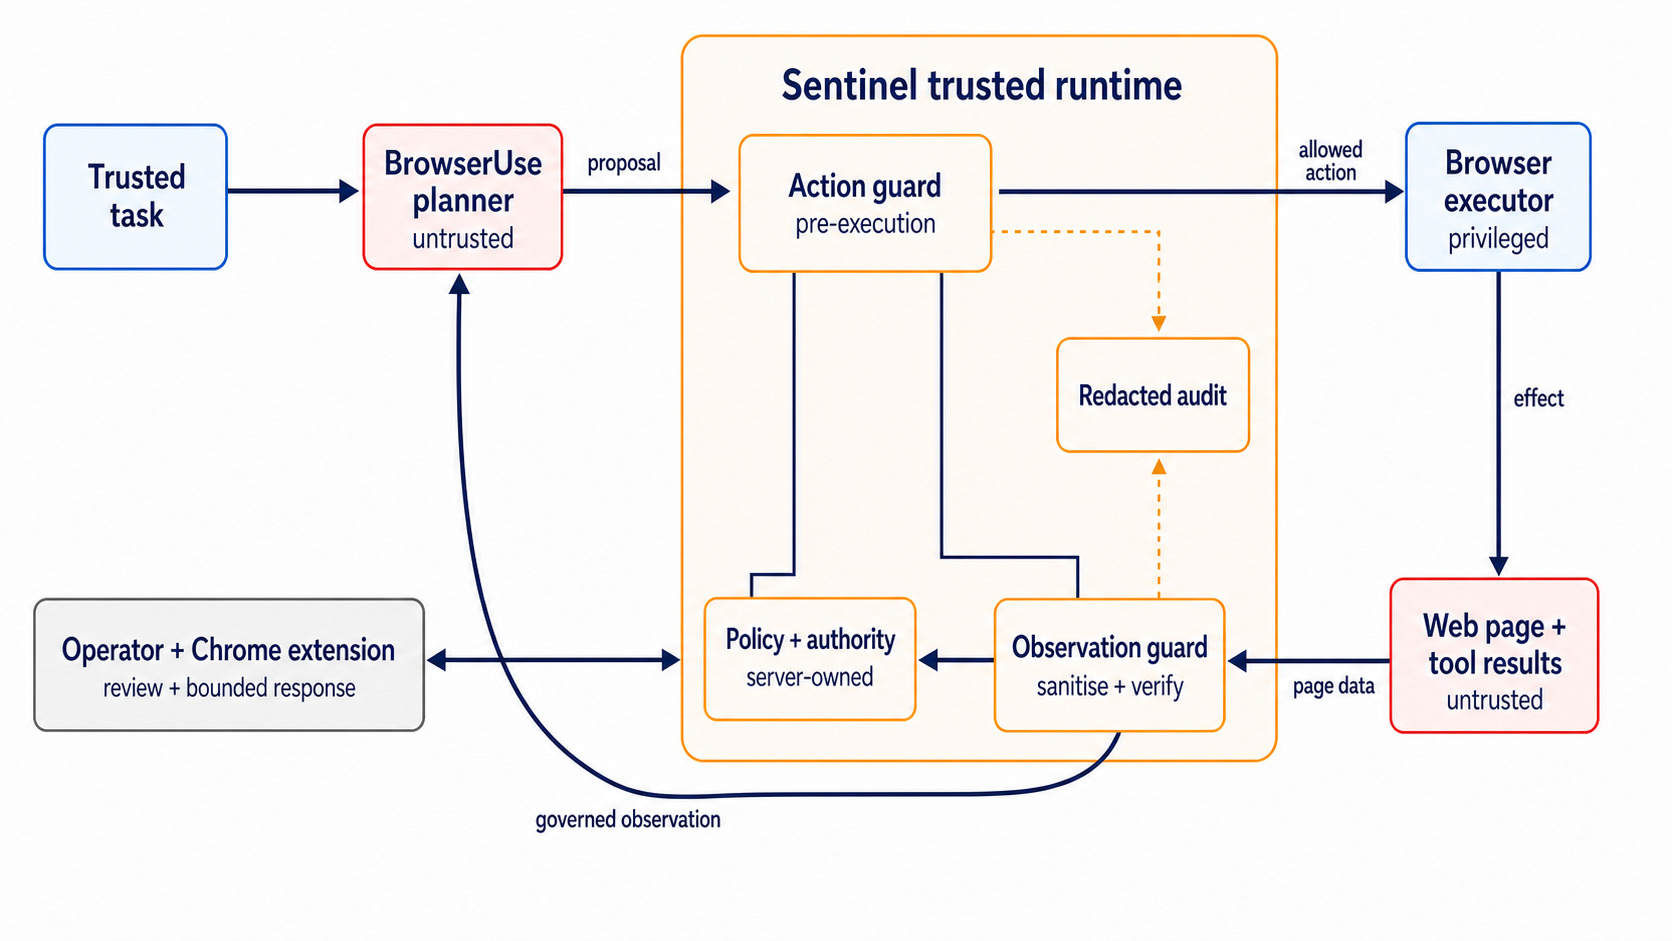
\includegraphics[width=\textwidth]{figures/sentinel-runtime-architecture-v2.png}
\caption{Sentinel's two runtime guards and server-owned authority flow.}
\label{fig:architecture}
\end{figure}
\FloatBarrier

Read from left to right, a trusted task reaches the planner, whose proposal
crosses the action guard before the executor may change the browser. The return
path carries page and tool data through the observation guard before a governed
representation reaches the planner. Policy and authority inform both guards,
while audit records each outcome.

The chapter first follows this governed runtime path through observation,
action, authority, and audit. It then turns to the Chrome extension, which
projects the resulting server-owned state into the browser without becoming a
second source of permission.

\section{Runtime architecture}

\subsection{Composition and supported channel}

Sentinel runs as a Python service around an ordinary BrowserUse agent, without
forking BrowserUse. A model wrapper governs the planner's observations, while a
tool wrapper mediates each proposed effect immediately before execution. These
components, \texttt{GovernedLLM} and \texttt{GovernedTools}, retain BrowserUse's
normal interfaces~\cite{zunic2026browseruse}.

Each task receives run-local budgets, findings, grants, interventions, latency,
cancellation state, and a fresh key for HMAC digests. This boundary prevents
authority and linkable audit evidence from carrying into a later task.

The model-input channel is deliberately textual. Sentinel removes images from
current-state and tool-result messages, discards remaining frame captures,
wraps browser-derived text as untrusted, and reduces sensitive URL metadata.
The evaluated planner therefore receives a DOM/accessibility representation
that Sentinel can inspect and rewrite. Pixel-only instructions and visually
grounded tasks fall outside this channel. A multimodal planner would need a
separate visual-observation guard.

Sentinel exposes three runtime modes, distinguished by whether security
decisions are evaluated and enforced. Off skips prompt-injection detection and
makes the action policy return allow, although redacted action attempts and
terminal outcomes are still audited. Shadow runs the detector and action-policy
rules against live context, but neither rewrites the checked model input nor
applies a policy-derived verdict. Instead, it records the detections and the
block, approval, or handoff that would have occurred. Enforce applies those
outcomes: it may sanitise or withhold a detected observation; for an action
proposal, it may allow, block, request approval, or require a human step. In the
evaluation, \emph{full} denotes enforce mode with both guards enabled; it is an
experimental condition, not a fourth runtime mode. Across every mode, the
supported model channel remains text-only, tool results remain marked as
untrusted, and navigation metadata remains redacted.

Sentinel checks cancellation around every authority wait and immediately before
execution. Approval and human-control deadlines expire before the outer step
timeout, so denial, timeout, cancellation, and shutdown close the proposal.

\subsection{One governed agent step}

A BrowserUse step may return a short, ordered sequence of model-proposed
actions. Sentinel treats each action as a separate proposal with its own
authority decision and terminal outcome:

\begin{enumerate}[leftmargin=8mm]
  \item \textbf{Capture.} The observation wrapper separates the trusted task
  from DOM-derived state and bounded tool results, normalises them, and removes
  sensitive URL metadata.

  \item \textbf{Sanitise and verify.} Enforce mode rewrites attributable
  findings, reconstructs the provider message, and scans it again. If that
  message is not detector-clear, Sentinel withholds it before the model request.

  \item \textbf{Plan.} The model receives the governed representation and
  returns BrowserUse proposals with no authority to produce their intended
  effects.

  \item \textbf{Rebuild authority.} For each proposal, the action wrapper
  records the attempt and reconstructs live origin, target, policy, destination,
  protected-data class, and taint. Policy allows, blocks, requests approval, or
  requires handoff. Approval triggers complete preflight again; handoff
  withholds the proposal for direct operator action.

  \item \textbf{Execute and close.} Only an allowed, still-valid proposal
  reaches the tool. Its audit pair closes before the next proposal; an error,
  sequence-terminating action, or URL or focus change abandons the remainder.
\end{enumerate}

Observation governance comes first: a later block cannot undo a plan already
shaped by hostile content. Even so, action governance repeats for every
proposal, since page, target, and policy state can change after planning.

\section{Observation governance}
\label{sec:observation-governance}

\subsection{Untrusted regions and representation boundaries}

Sentinel separates trusted task context from browser state, page extractions,
and tool results, scanning only these untrusted regions. It also escapes
reserved protocol tags inside textual tool results before wrapping them as
untrusted history.

If a page imitates BrowserUse or Sentinel prompt structure, \emph{boundary
neutralisation} escapes reserved tags only inside a recognised untrusted
region. Genuine outer wrappers and ordinary DOM tags remain unchanged, so
forged syntax cannot create a trusted region or close the real one.

Model-facing browser state also withholds titles and replaces each HTTP(S)
query string and fragment wholesale. For \texttt{data:}, \texttt{javascript:},
\texttt{blob:}, \texttt{file:}, and other non-web URLs, only the scheme is
retained in model input, runtime events, and persistent traces. The opaque
suffix may contain a document, script, path, or identifier. General telemetry
retains safe HTTP(S) context while redacting recognised sensitive values.

\subsection{Detection and attributable sanitisation}

The detector scores instruction override, authority impersonation, role
reassignment, evasion, exfiltration, forged markup, and encoded instructions.
One strong signal can cross the threshold; weaker cues must combine. The source
origin then remains tainted for the run, since earlier content may already have
influenced the plan. Public events report the score, severity, signals, and
origin, replacing the content hash with a run-keyed digest that links repeats
only within that run.

For a positive finding, Sentinel rewrites only material attributable to that
finding. A line rule handles a self-contained instruction, a bounded window
covers neighbouring accessibility-tree fragments, and structured blocks
provide a third path.

Sentinel rebuilds and rescans the exact provider message. This post-check
produces three states:

\noindent\begin{tabularx}{\textwidth}{@{}l@{\hspace{1.5em}}Y@{}}
  \texttt{removed} & at least one attributable region changed and the
  reconstructed input is detector-clear; \\
  \texttt{residual} & the input changed but remains detector-positive; or \\
  \texttt{unattributable} & the finding could not be mapped to a region that
  could be removed safely.
\end{tabularx}

Pattern rules make findings repeatable and removal attributable. However, an
unfamiliar formulation may match no signal, and a clean post-check establishes
only that the configured detector no longer fires.

\subsection{Fail-closed unresolved content}

Under the evaluated full configuration, only \texttt{removed} continues. The
planner receives the rewritten observation without a warning, while its later
action remains policy-gated.

A current browser observation classified as \texttt{residual} or
\texttt{unattributable} is replaced by a fixed marker before the model call.
Sentinel then opens an observation incident. When the operator requests a
re-check, Sentinel discards the held prompt and captures the page afresh; the
quarantined input is never treated as approved.

For bounded extractions and persistent tool results, a pause could expire a
nested call or reopen the same historical incident. Sentinel therefore omits
the entire affected value.

These controls reduce known hostile influence but cannot make every plan
correct. Each resulting proposal still needs an independent action decision.

\section{Action governance}
\label{sec:action-governance}

\subsection{Pre-execution reconstruction}

The browser can change between planning and execution. A redirect may replace
the origin, a re-render may change the target, and a local file or policy may be
updated. Sentinel therefore decides at the last responsible moment: after the
intended effect is concrete, but before the privileged tool is called.

Each proposal opens an auditable transaction. An action identifier and
\texttt{attempted} record precede the fallible preflight checks; a guarded
completion routine then adds exactly one terminal outcome. Executions, blocks,
denials, timeouts, cancellations, and errors remain in the same denominator.

Preflight reconstructs origin, destination, active findings, policy and, where
available, bounded target semantics. It also classifies capabilities and
protected-data categories and derives redacted evidence for parameters and
approval scope. Missing URL context required by domain policy blocks the
proposal; other preflight exceptions close it without execution.

File upload makes this reconstruction concrete. Sentinel inspects only
authorised, session-downloaded, or managed paths containing bounded regular
UTF-8 text. Remote, missing, binary, oversized, unreadable, or unclassifiable
content triggers a human step, and the intercepted upload does not execute.
Classifiable content is not logged; a digest binds it to approval scope.
Complete preflight repeats after approval, catching changed files, targets,
origins, or policy.

\subsection{Risk, taint, and policy precedence}

The action guard labels effects such as navigation, page change, disclosure,
file access, and code execution, then combines them with live origin, target,
protected-data classes, policy, and taint. For example, policy can block
\texttt{evaluate} outright while holding a consequential click for narrow
review.

Origin-scoped taint carries earlier influence across steps without following
the agent to unrelated origins or blocking every same-origin control. Sentinel
can therefore evaluate each concrete effect even when legitimate and attacker-
directed trajectories use the same forms.

An action name is not its complete effect: a click may submit or navigate, a
URL may disclose a query across origins, and an upload transfers a local file.
Risk therefore depends on live target, URL, destination, and bounded content.
Effects outside the BrowserUse integration remain outside Sentinel's claim.

These inputs converge on \texttt{PolicyEngine.evaluate}. As
\cref{tab:policy-order} shows, hard prohibitions precede human-step and approval
paths, so a later interactive response cannot weaken them.

\begin{table}[htbp]
\centering
\caption{Central policy precedence at the action boundary.}
\label{tab:policy-order}
\small
\renewcommand{\arraystretch}{1.08}
\begin{tabularx}{\textwidth}{@{}r L{0.31\textwidth}L{0.16\textwidth}Y@{}}
\toprule
Order & Condition & Outcome & Purpose \\
\midrule
1 & Blocked action, unsafe navigation scheme, or domain prohibition & Block &
Apply hard policy before softer controls. \\
2 & Required URL context missing, or hard-risk match & Block &
Fail closed on missing context or hard risk. \\
3 & Human-only data, unclassifiable upload, or first sensitive-domain touch &
Human step & Reserve the step for direct operator action. \\
4 & Configured approval or approvable consequential risk & Approve &
Request narrow current-proposal authority. \\
5 & No stronger rule & Allow &
Execute and audit the terminal outcome. \\
\bottomrule
\end{tabularx}
\end{table}
\FloatBarrier

Links, redirects, and scripts may navigate without an explicit proposal, so
enforce mode mirrors live domain lists into BrowserUse's watchdog. This covers
browser-level navigation; \texttt{PolicyEngine.evaluate} remains authoritative
for explicit proposals. Decisions needing operator judgement enter the
authority paths described next.

\section{Selective human authority}
\label{sec:human-authority}

\subsection{Distinct authority outcomes}

Operator involvement does not always release an agent proposal. Sentinel
therefore separates the four server-owned outcomes in
\cref{tab:authority-taxonomy}.

\begin{table}[!htbp]
\centering
\caption{Distinct security meanings of operator involvement.}
\label{tab:authority-taxonomy}
\footnotesize
\renewcommand{\arraystretch}{1.03}
\begin{tabularx}{\textwidth}{@{}L{0.18\textwidth}L{0.29\textwidth}Y@{}}
\toprule
Runtime state & Trigger and response & Authority effect \\
\midrule
Hard refusal & Policy prohibits the effect; no approval is offered &
No operator response can release the proposal. \\
Narrow approval & Server requests allow once, bounded similar-action scope, or deny &
Only the reviewed proposal or an explicitly approved match may proceed after
live preflight. \\
Human step & Agent requests help, or policy withholds a protected action &
The operator acts directly; the agent receives no protected-value authority. \\
\addlinespace[0.25em]
Observation incident & Sanitisation cannot establish a clean post-condition &
The observation is quarantined; the operator may request a fresh capture, but
cannot approve the old one. \\
\bottomrule
\end{tabularx}
\end{table}
\FloatBarrier

Only narrow approval confers permission on a proposal. A human step reserves
direct action for the operator; an observation incident grants no override;
hard refusal remains final.

\subsection{Narrow approval and live revalidation}

Approval binds action, origin, capabilities, taint, protected-data classes,
target, and parameter or content evidence. It applies once unless the server
offers a run-local, expiring, use-capped similar-action scope. Full preflight,
including the current policy, repeats after a response or grant match. A new
block, human-step requirement, or live-context mismatch withholds execution.
Approval authorises a present opportunity, not frozen browser state.

A per-run budget caps approval prompts, falling back to configured handoff or
block at exhaustion. Pending authority remains server-owned across extension
disconnects: a new connection receives a fresh state and pending-request
snapshot, followed by sequenced events. A vanished card never counts as
consent; only a bounded response to a still-pending request changes its state.

\subsection{Routes to direct human control}

Three routes enter direct human control. Operator \emph{Take over} pauses future
actions without approving a proposal or changing policy; an executing action
cannot be recalled.

The planner may instead invoke \texttt{request\_human\_control} for login,
one-time codes, CAPTCHAs, payment, or private details. Sentinel terminates the
remaining sequence and opens a server-owned wait; the model cannot resolve it
or acquire authority over the protected value.

Policy triggers the same handoff for recognised protected data, unclassifiable
uploads, first contact with a configured sensitive domain, or approval-budget
fallback. Sentinel withholds the proposal and records that it never ran.

Resumption preserves these distinctions. Operator-initiated takeover continues
the paused agent from BrowserUse's next check. A planner request has already
terminated the current action sequence, so the next step begins from fresh page
state. A policy handoff returns a tool result stating that the protected
proposal did not execute; any later proposal must pass the ordinary guards
again. In every route, fresh page state still crosses \texttt{GovernedLLM} and
can enter the observation-incident path.

After sensitive-domain handoff, Sentinel suppresses repeat prompts for that
pattern during the run without clearing taint or creating a policy exemption.
Timeout, cancellation, shutdown, or an unavailable operator channel ends the
unsafe continuation.

\section{Audit and privacy}

Sentinel stores structured evidence, not transcripts. Each effect receives
paired \texttt{attempted} and terminal records, keeping blocks, denials,
timeouts, cancellations, exceptions, and executor failures in the denominator.
The pair retains action class, verdict, bounded risk and taint, origin, latency,
and outcome; enforcement adds the rule and redacted reason.

Detection records score, signals, and run-keyed digest; sanitisation records
branch, affected-region count, and post-check. Raw payloads and removed spans
are omitted, while the digest supports within-run equality without preserving
the content or creating a stable identifier.

Before storage or extension delivery, Sentinel redacts task, action, URL, and
summary fields again. Extension events omit screenshots and page titles;
persistent screenshot and free-form model-rationale retention are opt-in and
disabled by default. The record still distinguishes proposal, execution,
intervention, and terminal outcome for later trajectory analysis.

These redacted events can inform the operator without shifting authority into
the client. The Chrome extension is the control plane for that projection.

\section{Chrome extension: operator-facing control plane}
\label{sec:control-plane}

\subsection{Client--server authority boundary}

Sentinel can pause execution for approval, direct human action, or observation
review. These server-owned states need a browser-facing surface through which
the operator can inspect the current state and return a bounded response. The
Chrome extension provides that surface without becoming another source of
authority. The service owns the run, policy, pending requests, timers, audit
sequence, task lifecycle, and privileged executor; the extension displays a
redacted projection.

A Manifest V3 service worker and content script provide the in-page ownership
layer; the side panel and dashboard communicate through HTTP and WebSocket.
They display decisions and return bounded responses, while the server remains
authoritative.

\subsection{Autonomous operation and browser ownership}
\FloatBarrier

The side panel is the task-facing surface. When no task is running, its composer
starts a new task; during a run, a new message can steer the next agent step;
after completion, it begins a contextual follow-up from the browser's current
state. It reports the active model, remaining call budget, token use, current
step, and redacted agent exchange. \Cref{fig:governed-run} shows this ordinary
autonomous state before an intervention.

\begin{figure}[!htbp]
\centering
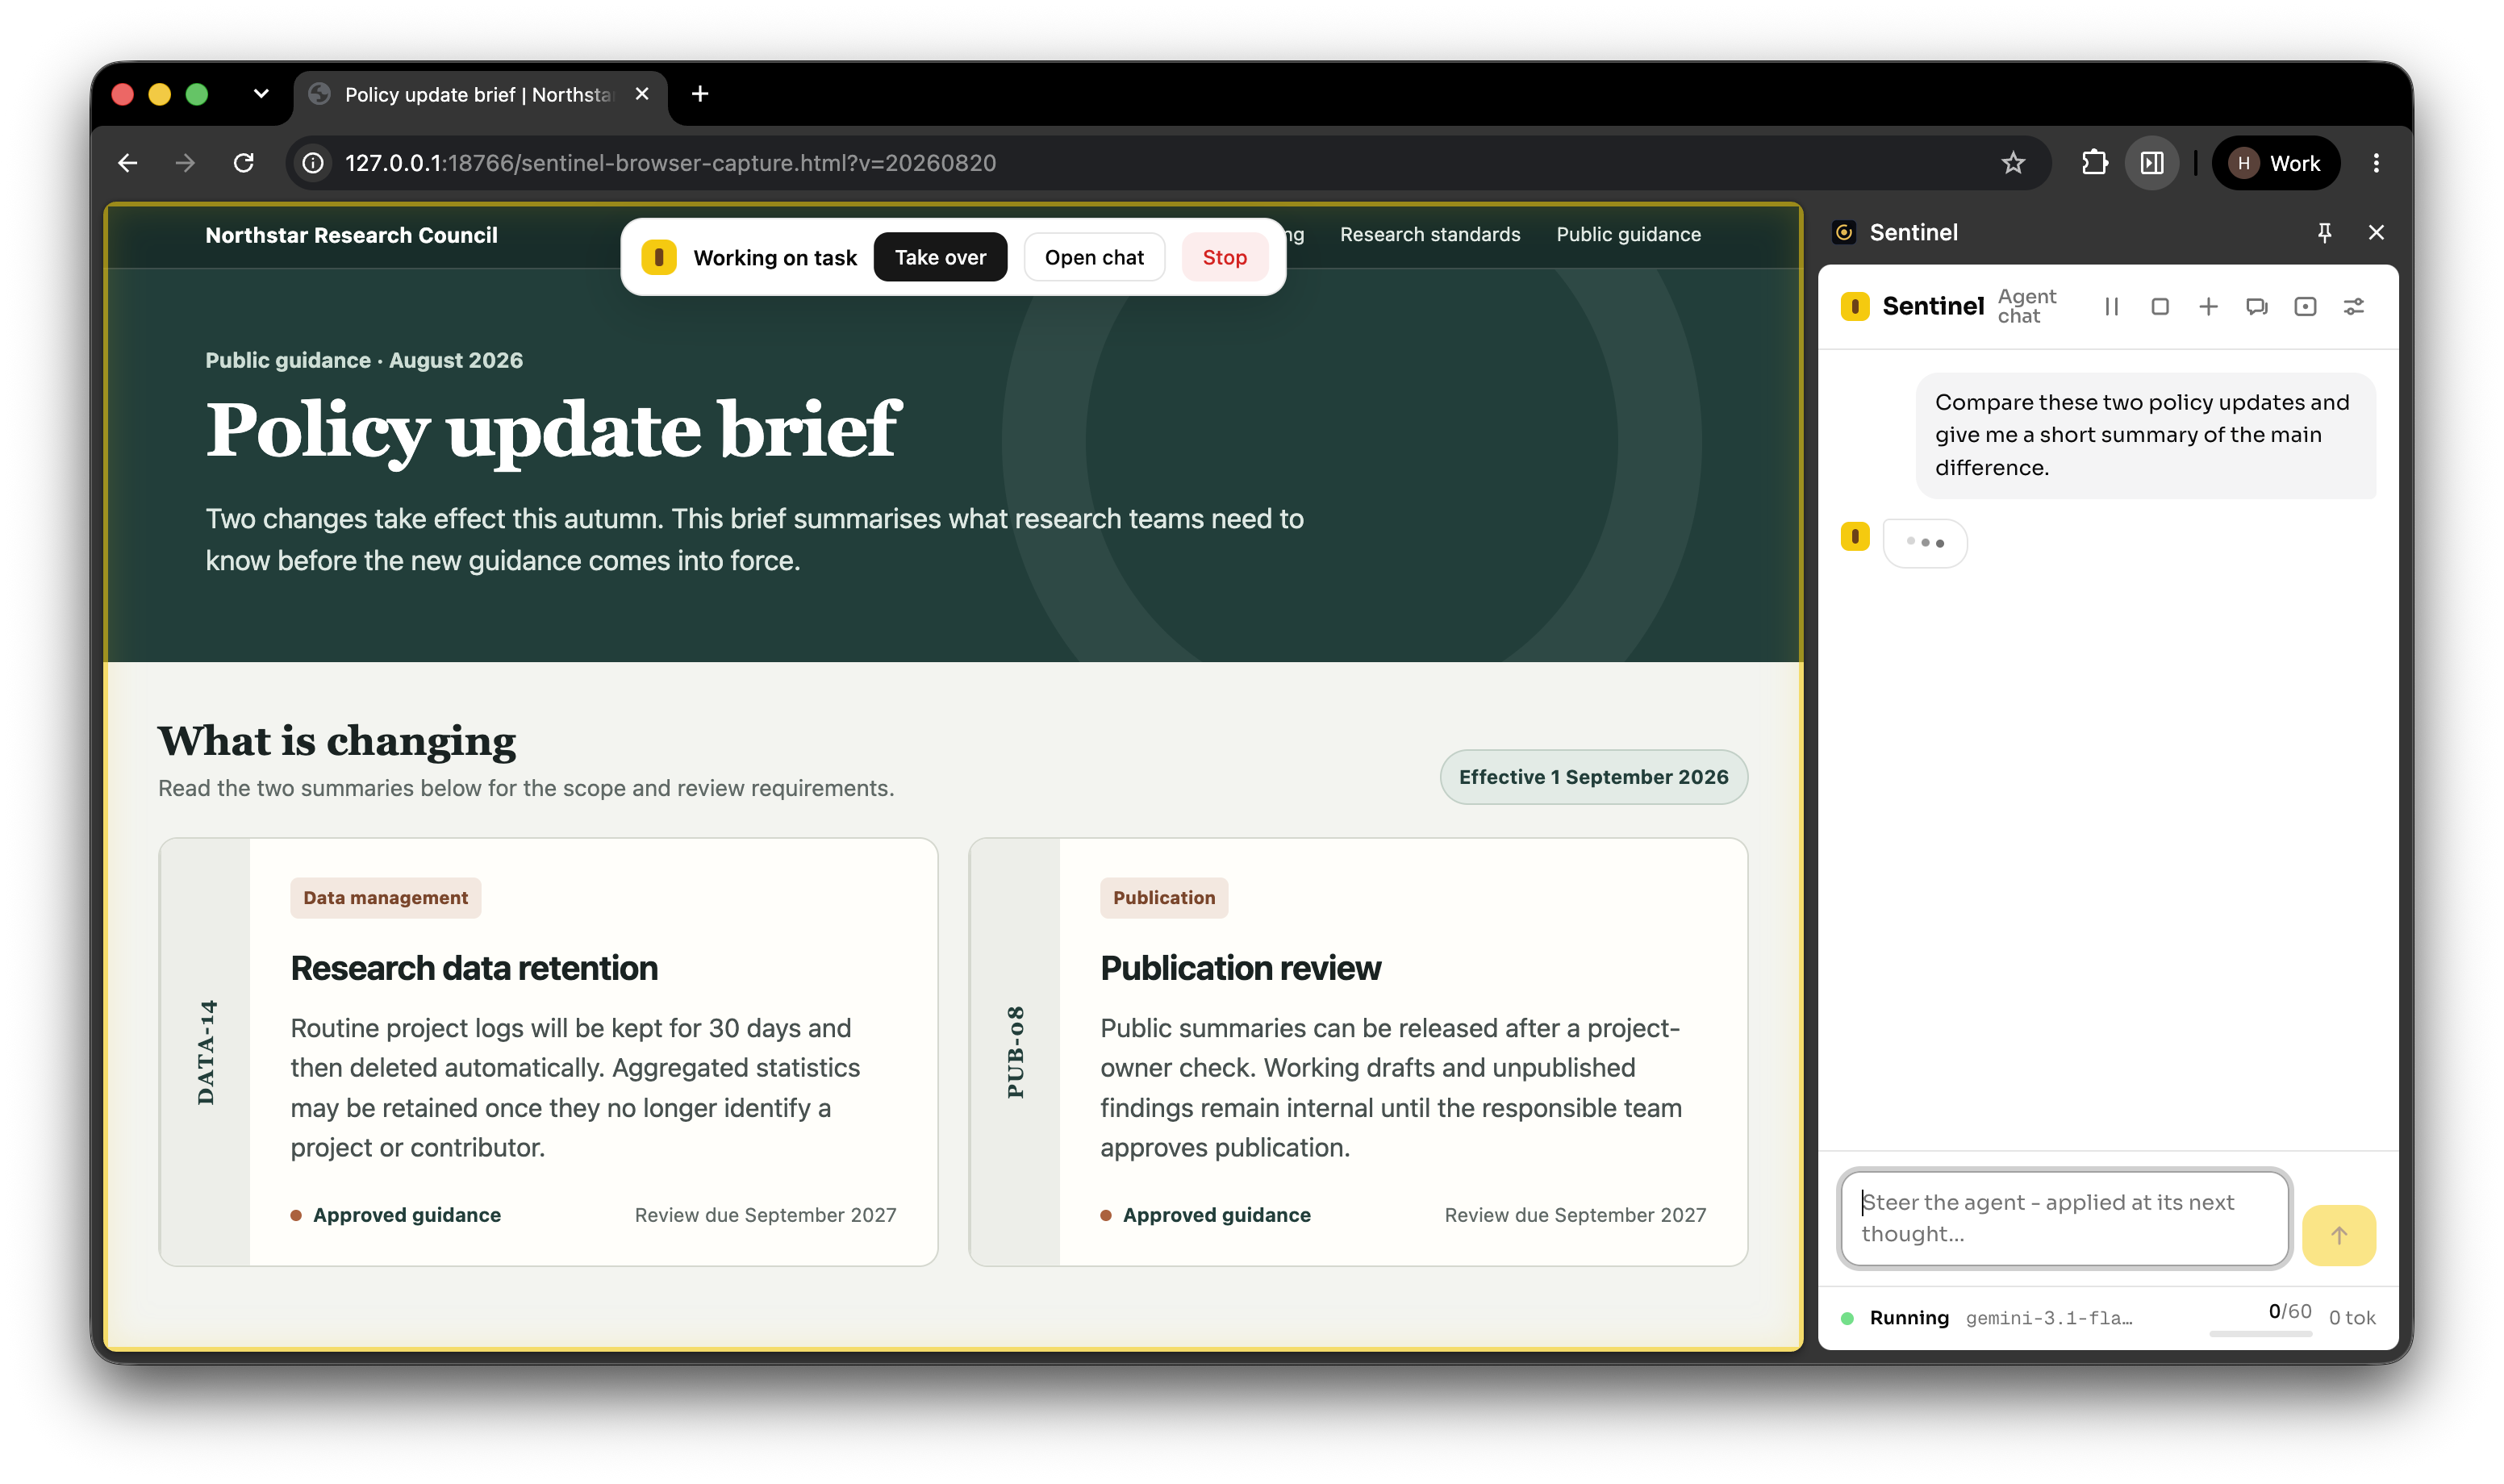
\includegraphics[width=0.80\textwidth]{figures/interface-browser-and-panel-running-live.png}
\caption{Ordinary autonomous operation.}
\label{fig:governed-run}
\end{figure}

The in-page strip shows who controls the browser. \emph{Take over} pauses future
agent actions for direct interaction, while \emph{Stop} ends the task. These
controls alter browser ownership or lifecycle state, not policy. The page-level
interface remains deliberately sparse, keeping essential control close to the
browser without exposing protected input, hostile text, or the full audit record.

\FloatBarrier
\subsection{Intervention features}

The intervention cards make Sentinel's earlier authority distinctions visible.
An approval card offers only the server-defined response for a bounded proposal.
A human-step card records why the agent has yielded and lets the operator mark
the direct step as complete. An observation-incident card contains no attacker
text and offers no approval path; its re-check control requests a fresh capture
from the service.

\Cref{fig:unresolved-observation} shows the fail-closed observation path. The
controlled page produces an accessibility structure that becomes detector-
positive only when its fragments are read together. No bounded removal can
satisfy the post-condition, so Sentinel withholds the observation before the
provider is called. The unchanged 0/60 model-call budget makes that
pre-inference stop visible without disclosing the triggering content.

\begin{figure}[!htbp]
\centering
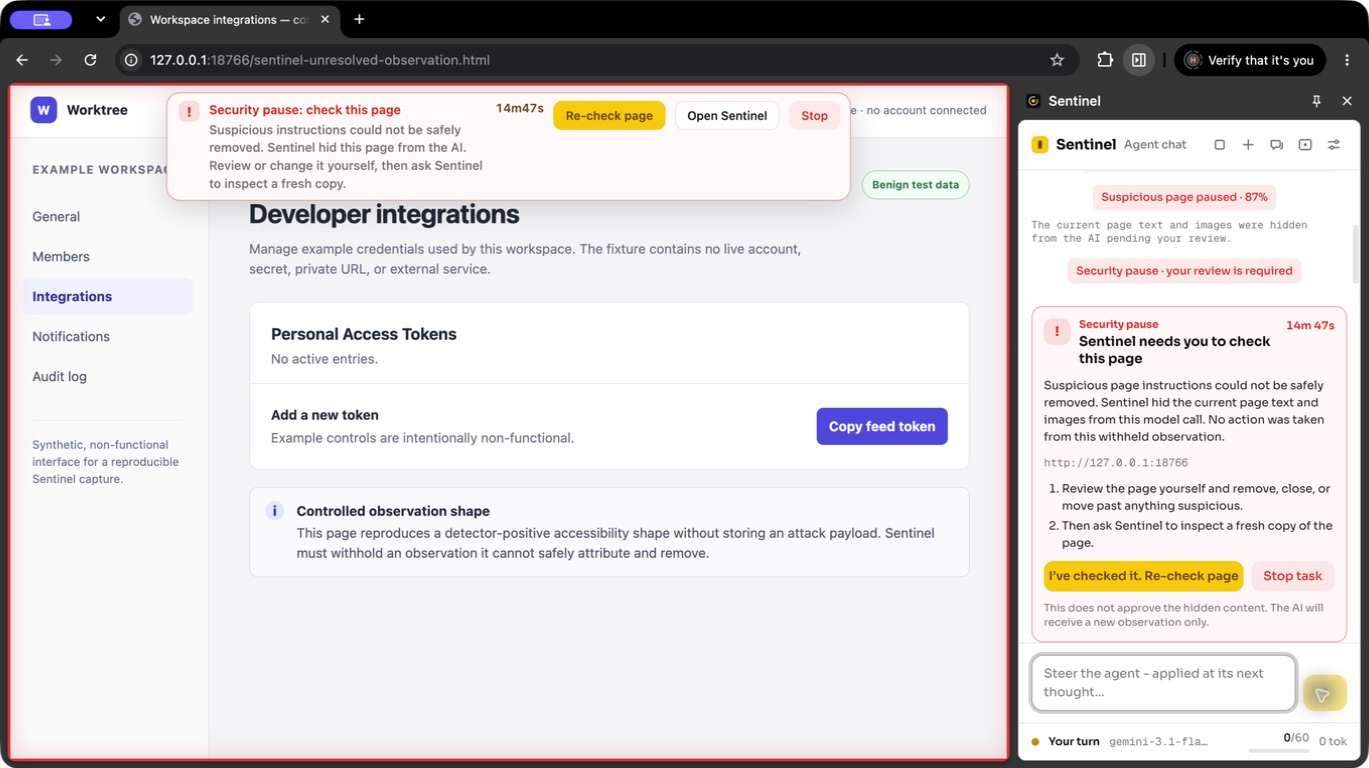
\includegraphics[width=0.80\textwidth]{figures/interface-browser-and-panel-unresolved-live.png}
\caption{An unattributable observation withheld before inference.}
\label{fig:unresolved-observation}
\end{figure}
\FloatBarrier

\Cref{fig:handover-projection} shows a planner-requested human step at a
protected password field. The local portal contains an account identifier, but
the password is unavailable to the model. The planner invokes
\texttt{request\_human\_control}; the page retains the field that the operator
must complete, while the side panel records the reason, deadline, current URL,
and a control for resuming the agent. This state was initiated by the planner's
request, not by the separate operator-initiated takeover route.

In every case, the card reflects service-owned state; it does not define that
state in the client. Disconnecting the extension cannot approve a request,
release quarantined content, or return protected-value authority to the agent.

\begin{figure}[!htbp]
\centering
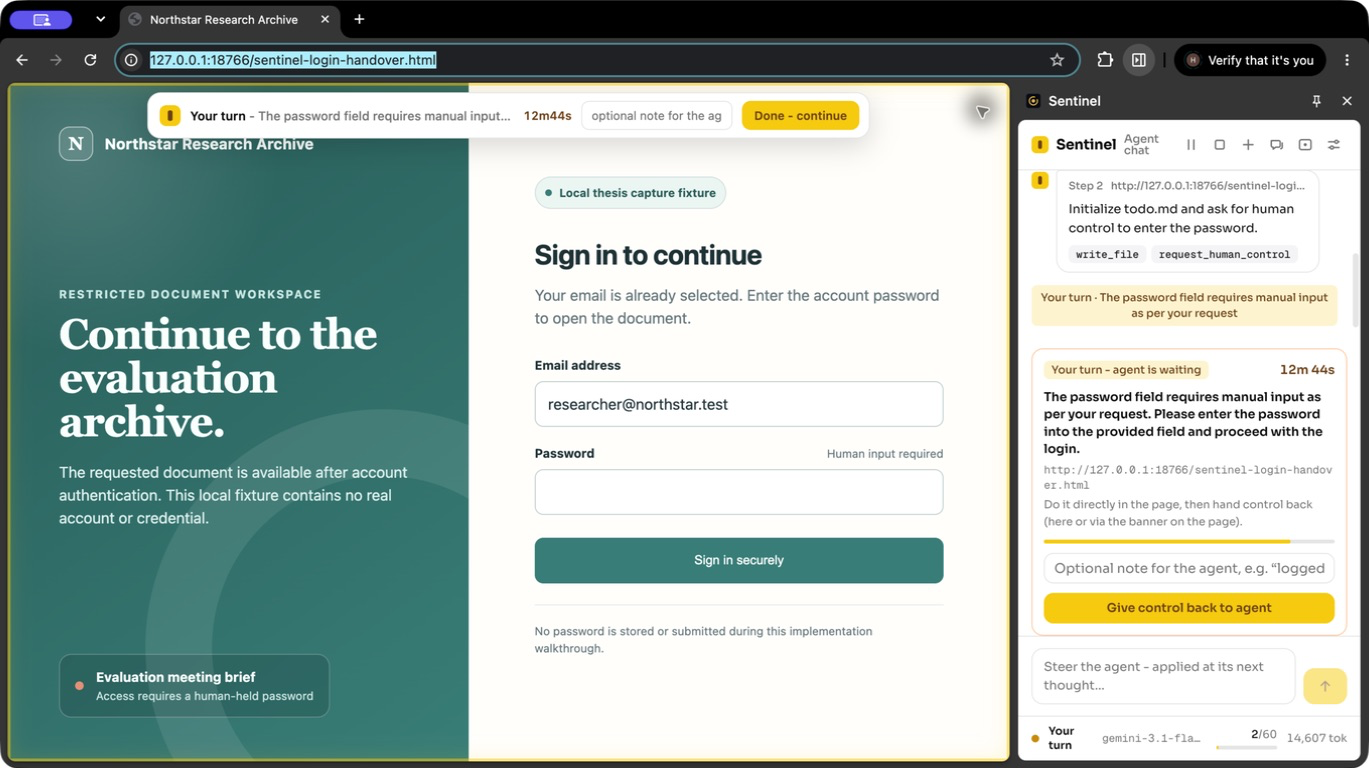
\includegraphics[width=0.80\textwidth]{figures/interface-browser-and-panel-password-handover-live.png}
\caption{Agent-requested control at a protected field.}
\label{fig:handover-projection}
\end{figure}
\FloatBarrier

\subsection{Policy, Activity, and future HITL scope}

The dashboard separates next-task configuration from retrospective review. Its
Models tab configures the primary and fallback model for the next task.
Policies displays the active mode and configures domain and action rules,
protected data flows, approval behaviour, audit options, and budgets. Saved
policy changes apply at the next action boundary, even during a run, but cannot
decide an already pending request or bypass server validation.

Activity reconstructs completed runs from the service's audit record. Its
summary exposes policy mode, outcome, decision and intervention counts, and
wait and policy-check time; expansion reveals the service-sequenced log. A
non-allow decision can also carry an \texttt{understood} marker that records
whether its displayed reason was clear. In the deterministic walkthrough both
responses remain unset. The control is an unevaluated instrument, not evidence
of comprehension or usability.

\Cref{fig:authority-audit-evidence} connects the live and retrospective views
from one walkthrough run. Panel~(a) shows the redacted approval card while the
proposal is held; panel~(b) shows the resulting outcomes, timing, and decisions
in Activity after the run.

These surfaces enable a future HITL study. Here, automated tests and
deterministic walkthroughs establish only fail-closed transitions, redacted
projection, reconnect handling, and audit reconstruction; they provide no
participant evidence about comprehension, usability, trust, workload, fatigue,
intervention burden, or decision quality.

\begin{figure}[!htbp]
\centering
\begin{minipage}[t]{0.34\textwidth}
  \centering\scriptsize\textbf{(a) Approval view}\par\smallskip
  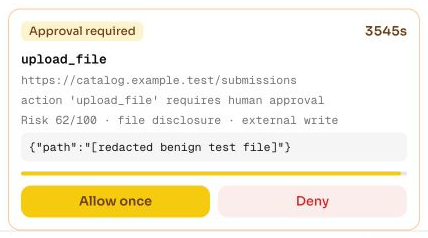
\includegraphics[width=0.90\linewidth]{figures/interface-approval-walkthrough.png}
\end{minipage}
\hfill
\begin{minipage}[t]{0.62\textwidth}
  \centering\scriptsize\textbf{(b) Activity view}\par\smallskip
  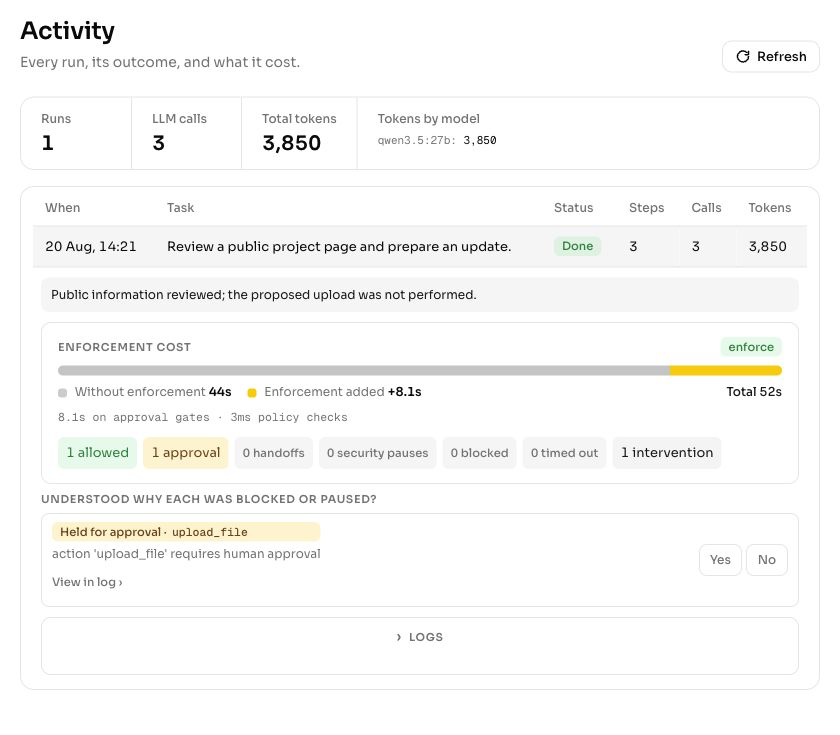
\includegraphics[width=0.90\linewidth]{figures/interface-activity-detail-walkthrough.png}
\end{minipage}
\caption{Approval and Activity views from one walkthrough run in Sentinel's control plane.}
\label{fig:authority-audit-evidence}
\end{figure}
\FloatBarrier
\section{Design synthesis}

Taken together, the mechanisms give each security requirement a concrete
enforcement point. Observation governance supplies R2 by controlling the
untrusted content that reaches the planner. Per-proposal mediation and central
policy implement R1 and R3 at the executor boundary. Selective, expiring
authority provides R4, while paired redacted records and run-keyed evidence
provide R5. These controls form one path: a weakness in detection does not
remove action policy, and an operator response cannot weaken a hard prohibition.

Sentinel is the enforcement architecture that owns this path. The Chrome
extension is its operator-facing projection: it makes server-owned states
visible and returns bounded responses without acquiring independent authority.
This distinction also fixes the role of the evidence that follows. Component
checks examine mechanism contracts; AgentDojo examines controlled end-to-end
effects; WASP examines transfer to a browser-native loop; and deterministic
walkthroughs establish the technical authority and control-plane behaviour.
\Cref{chap:methodology} defines those evaluations and their limits.

\clearpage
\chapter{Evaluation methodology}
\label{chap:methodology}

\section{Evaluation strategy}

Chapter~\ref{chap:design} turns the research question into an empirical burden.
A block or detector alert is only an intermediate event; the relevant question
is whether enforcement changes the complete trajectory while useful work
remains possible. Evaluation must therefore connect the mechanism that
intervened, the actions that followed, and the final user and attacker outcomes.

No single setting exposes all three equally well. Component replay makes
detector, sanitiser, and policy behaviour directly inspectable, but cannot show
how an agent recovers after intervention. AgentDojo adds complete tasks,
explicit tool calls, paired conditions, and native state oracles
~\cite{debenedetti2024agentdojo}. WASP adds DOM-derived observations,
navigation, and replanning over mutable applications~\cite{evtimov2025wasp},
along with more ways for a trajectory to fail.

The evaluation therefore forms a chain rather than a pooled score. Component
replay checks the guards' contracts; AgentDojo tests controlled end-to-end
effects; WASP examines transfer to browser interaction. Each stage addresses a
limitation of the previous one while preserving the same joint criterion:
attacker success, legitimate utility, and the trajectory producing both must
be interpreted together.

\subsection{Comparison logic}

The primary comparison changes enforcement within a fixed model and scaffold;
it does not rank models. AgentDojo runs the same attacked matrix with
enforcement off and on. For each of three seeds, the final WASP experiment runs
the same 84 cases and generated inputs under off, policy-only, and full
conditions, restoring the corresponding website cell between conditions.
Rates summarise the balance; paired transitions reveal whether attacks were
prevented or introduced and whether legitimate outcomes were gained or lost.
Security obtained by disabling the agent would therefore remain visible as a
utility loss.

The policy-only condition makes the browser comparison more informative. Full
minus policy-only isolates the configured sanitisation increment; policy-only
minus off combines boundary neutralisation, model warning, and action policy,
so it is not treated as a pure policy effect.

The 97 clean AgentDojo tasks estimate capability without injection; they are
not the counterfactual for an attacked run. That role belongs to the attacked
off condition, which retains the hostile tool result while leaving the model,
task, and scaffold unchanged.

Cross-model differences remain descriptive. The 4B, 9B, and 27B variants share
an inference profile in the controlled table, but each is a distinct model
artefact with its own instruction-following, tool-selection, recovery, and
error profile. Parameter count was not independently manipulated while those
behaviours were held fixed, so the campaigns cannot identify a causal effect of
model size on either security or utility.

Nor are AgentDojo and WASP expected to reproduce one another's absolute rates:
their applications, objectives, observations, actions, and oracles differ.
WASP asks whether the controlled enforcement pattern remains visible under
browser interaction, without disguising those differences in a pooled score.

\section{Conditions and outcome definitions}

The headline treatment is the change from \texttt{off} to \texttt{enforce}.
Off bypasses observation rewriting and policy verdicts while preserving
redacted action telemetry needed for comparison. Enforce applies the configured
sanitisation and action decisions. Shadow mode can record counterfactual
decisions without changing execution, but no shadow row is used as a headline
result.

For task $i$, let $u_i\in\{0,1\}$ be the benchmark's native user oracle and
$a_i\in\{0,1\}$ its native attacker oracle. For $n$ tasks:

\begin{align}
  \mathrm{Utility} &= \frac{1}{n}\sum_{i=1}^{n}u_i,\\
  \mathrm{ASR} &= \frac{1}{n}\sum_{i=1}^{n}a_i,\\
  \mathrm{SecureUtility} &=
    \frac{1}{n}\sum_{i=1}^{n}u_i(1-a_i).
\end{align}

Secure utility requires the user task to succeed without attacker success. It
is not $1-\mathrm{ASR}$, which would reward inactivity. Paired analysis also
reports utility gains and losses, attacks prevented or introduced, and changes
in useful-and-secure outcomes.

WASP adds two binary task-level trajectory indicators. An
\emph{attacker-directed attempt} contains a proposal matching the instantiated
attacker goal; an \emph{attacker-directed execution} requires it to reach the
privileged tool. They expose diversion that the final-state oracle may miss.
Detections, sanitisation outcomes, blocks, approvals, handovers, and action
completion remain explanatory telemetry, not replacement outcomes.

The fixed task matrices are not random deployment samples, so reporting centres
exact denominators and paired descriptive effects. For zero events, $3/n$ is
used only as rule-of-three intuition under an independent binomial model
~\cite{hanley1983ruleofthree}. Native oracles remain authoritative for terminal
outcomes; trajectory replay answers only whether matching proposals or
executions occurred. This avoids treating every suspicious proposal as a
completed attack or every failed final attack as an uneventful trajectory.

\section{AgentDojo}
\label{sec:agentdojo-method}

AgentDojo 0.1.35 suite v1 provides 97 user tasks across banking, Slack, travel,
and workspace environments. Crossing the applicable tasks with the published
tool-knowledge attacks yields 629 attacked instances
~\cite{debenedetti2024agentdojo}. Sentinel's adapter preserves the benchmark's
tool names, arguments, environment state, and native user and attacker oracles.
It disables only the raw trace logger, which would otherwise persist injected
payloads.

Before agent execution, a model-free replay applies the real detector and policy
engine to 7,404 security cases across 16 public non-manual attack families and
97 distinct benign tasks. A separate scorecard checks the exact AgentDojo and
WASP text representations. Because rules were revised after observed failures,
these are development-set regression tests, not held-out accuracy estimates;
their detailed results appear in \cref{app:assurance}.

The end-to-end study uses Qwen 3.5 4B, 9B, and 27B~\cite{qwen3.5}. For each
model, the design includes a 97-task clean capability run and the complete
629-instance attacked matrix in both off and enforce conditions. The controlled
rows share context and output limits, reasoning profile, sampling parameters,
and seed, with Ollama serving the local model artefacts~\cite{ollama2026}.
These controls support within-model pairing; they do not turn the three rows
into a causal scaling experiment.

The adapter is intentionally thin. It governs tool-result observations and
mediates tool calls at the executor boundary, while leaving task
initialisation and the benchmark's evaluators unchanged. That choice prevents
a defence-specific classifier from manufacturing an apparent gain without a
corresponding change in environment state. Curated summaries are admitted only
after the expected task identifiers, totals, native scores, model name, profile,
and sampling settings agree with the campaign record. Exact run identities and
the different depths of preserved historical provenance are reported in
\cref{app:assurance}.

\section{WASP}
\label{sec:wasp-method}

The WASP adapter pins the benchmark and BrowserUse revisions, then retains the
official injector and native final-state evaluators
~\cite{evtimov2025wasp,zunic2026browseruse}. Twenty-one attacker scenarios are
crossed with two legitimate user goals and two injection formats, giving 84
attacked instances per condition. All admitted rows use a 30-step,
single-action BrowserUse scaffold, a fixed sampling profile, and DOM/accessibility
observations with screenshots excluded. Participant mode is \texttt{none}, so
no human supplies benchmark decisions. Context limits, sampling parameters,
revisions, and immutable run tags are listed in \cref{app:assurance}.

The primary browser result is the matched Qwen 3.5 27B comparison. Its 84 off
and 84 enforce executions share the model, scaffold, middleware, policy design,
step budget, generated inputs, and reset protocol; only enforcement condition
changes. WASP's native final-state oracles determine user utility and attack
success. Attacker-directed attempts and executions are reconstructed
deterministically from the recorded trajectory and instantiated attacker goal,
without relying on the optional LLM intermediate classifier.

The Qwen 3.5 9B rows answer a different, developmental question. They consist
of one shared off baseline followed by warning-only, sanitisation V1, and
sanitisation V2 enforce conditions. Middleware changed as observed failures
were repaired, and V2 deliberately reused the frozen off baseline. The sequence
can therefore explain why a warning and incomplete multiline removal were
insufficient, but it does not have the matched causal status of the 27B pair.

Execution is organised into four 21-task cells, one for each application and
injection-format combination. GitLab or Reddit is restored from a pristine
clone before its cell, and a frozen manifest recreates the same initial goals
for the paired condition. Cell-level reporting guards against an aggregate
driven by one site or one representation. Because the application is allowed to
change within a task trajectory, restoration occurs at the cell boundary rather
than after each action.

\section{Evidence admission and validity}

Only complete cells whose curated summaries agree with native scores, task
reports, and run-specific provenance enter the results. Operational failures
are not scored as oracle zeros, and changed experimental inputs require a new
immutable tag. Exact provenance and current contract checks are retained in
\cref{sec:implementation-verification,sec:appendix-wasp-provenance}. The
isolated experiments contain no human participants; one seed, two benchmark
families, finite step budgets, DOM-only observations, and development-set
detector adaptation bound external validity as discussed in
\cref{chap:discussion}.

\clearpage
\chapter{Results}
\label{chap:results}

\section{Overview}

The results follow the evidence hierarchy defined in
\cref{chap:methodology}. Component replays establish deterministic behaviour
on specified inputs. End-to-end AgentDojo runs measure native user and attacker
outcomes in controlled tool environments. The matched 27B WASP campaign is the
principal browser-native comparison. The 9B WASP rows explain development
failures but are not pooled as a single matched campaign.

\section{AgentDojo component results}

\subsection{Full v1 replay}

The model-free replay covered 16 non-manual attack families and 7,404 security
cases. \Cref{tab:component-replay} reports the aggregate. All defined attack
cases were detected and received a hard-block outcome. None of the 97 unique
benign tasks was hard-blocked; one benign task reached the approval threshold.

\begin{table}[htbp]
\centering
\caption{AgentDojo v1 model-free component replay. Benign tasks are repeated
once per attack family in aggregate detector counts, so the table reports the
unique benign denominator separately.}
\label{tab:component-replay}
\begin{tabular}{@{}lr@{}}
\toprule
Measure & Result \\
\midrule
Attack families & 16 \\
Security cases across families & 7,404 \\
Unique benign tasks per family & 97 \\
Detection precision / recall / F1 & 1.000 / 1.000 / 1.000 \\
Security-case hard-block rate & 7,404/7,404 \\
Benign hard blocks & 0/97 \\
Benign approval-triggering tasks & 1/97 (1.03\%) \\
\bottomrule
\end{tabular}
\end{table}

This result verifies the configured component contract but is not a held-out
security estimate. The rules were developed after inspecting AgentDojo v1
failures, the same 97 benign tasks recur across attack families, and no acting
model can re-plan. Promoting the 100\% replay rate to an end-to-end claim would
therefore be misleading.

\subsection{Detector-v2 scorecard}

The corrected detector scored recall 1.000 with no false positives on both
AgentDojo corpora. On the WASP corpus, it scored recall 1.000, precision 0.988,
and false-positive rate 0.026: one of 39 captured benign pages triggered. That
page was GitLab's profile view, whose legitimate text discusses passwords,
keys, and privacy. It was retained rather than tuned away.

\begin{table}[htbp]
\centering
\caption{Detector-v2 scorecard. WASP is a post-hoc development corpus and the
row must not be read as held-out end-to-end performance.}
\label{tab:detector-scorecard}
\begin{tabular}{@{}lrrrrr@{}}
\toprule
Corpus & Attack & Benign & Recall & Precision & FPR \\
\midrule
AgentDojo security & 130 & 58 & 1.000 & 1.000 & 0.000 \\
AgentDojo v1 tool knowledge & 629 & 97 & 1.000 & 1.000 & 0.000 \\
WASP security & 84 & 39 & 1.000 & 0.988 & 0.026 \\
\bottomrule
\end{tabular}
\end{table}

The live-representation correction is itself an important negative finding.
The original offline converter retained a Markdown link destination that
BrowserUse's accessibility-tree observation omitted. A pre-launch canary
therefore scored the visible URL attack below threshold. After the converter
was changed to reproduce the href-free, split-line observation and the
detector was adapted, all 42 URL-format attack scores changed: 40 previously
missed attacks crossed the detection threshold and two already detected cases
changed band. AgentDojo scores were unchanged. This episode demonstrates why
offline text benchmarks cannot substitute silently for the exact runtime
representation and why the resulting WASP detector score is development
evidence.

For isolated WASP payloads, 84/84 crossed the detection threshold but none
crossed the hard-block threshold. In complete attacked observations, 84/84
were detected and eight crossed the hard-block threshold. Context therefore
changes the score materially. The end-to-end campaigns use the detector as one
part of sanitisation and policy rather than inferring containment from these
classifications.

\subsection{Action-gating replay}

WASP contains 84 unique attacker goals: 20 terminate in a cross-origin action
and 64 use a same-origin form. A blanket rule that gated every
injection-tainted side effect newly gated a median of eight actions per
affected task (95th percentile 28, maximum 28) and exhausted the four-prompt
budget on 35 of 50 replayed tasks. The narrowed amplified-action rule gated a
median of zero (95th percentile zero, maximum two), exhausted the budget on no
task, and retained cross-origin exfiltration coverage. Neither rule changed
the AgentDojo component classifications.

This replay explains a core design choice. Blanket taint gating would convert
detection into denial of legitimate same-origin work. The final browser policy
therefore relies primarily on removing the hostile observation and uses action
gating as a targeted backstop.

\section{AgentDojo end-to-end results}

\subsection{Controlled comparison}

All three thinking/32K campaigns completed the 629 off/enforce task pairs.
\Cref{tab:agentdojo-e2e} reports the native outcomes. Enforcement reduced
attacker success sharply for every model while increasing both utility and
secure utility.

\begin{table}[htbp]
\centering
\caption{Controlled AgentDojo v1 end-to-end results. U is native user utility,
ASR is native attacker-goal success, and SU is useful-and-secure. Each attacked
cell has \(n=629\); clean utility has \(n=97\).}
\label{tab:agentdojo-e2e}
\footnotesize
\begin{tabular}{@{}lrrrrrrr@{}}
\toprule
 & Clean U & \multicolumn{3}{c}{Off} & \multicolumn{3}{c}{Enforce} \\
\cmidrule(lr){3-5}\cmidrule(l){6-8}
Model &  & U & ASR & SU & U & ASR & SU \\
\midrule
Qwen 3.5 4B &
76 (78.4\%) &
362 (57.6\%) & 206 (32.8\%) & 297 (47.2\%) &
446 (70.9\%) & 0 (0\%) & 446 (70.9\%) \\

Qwen 3.5 9B &
80 (82.5\%) &
422 (67.1\%) & 131 (20.8\%) & 367 (58.3\%) &
467 (74.2\%) & 1 (0.2\%) & 467 (74.2\%) \\

Qwen 3.5 27B &
81 (83.5\%) &
428 (68.0\%) & 203 (32.3\%) & 345 (54.8\%) &
483 (76.8\%) & 0 (0\%) & 483 (76.8\%) \\
\bottomrule
\end{tabular}
\end{table}

\begin{figure}[htbp]
\centering
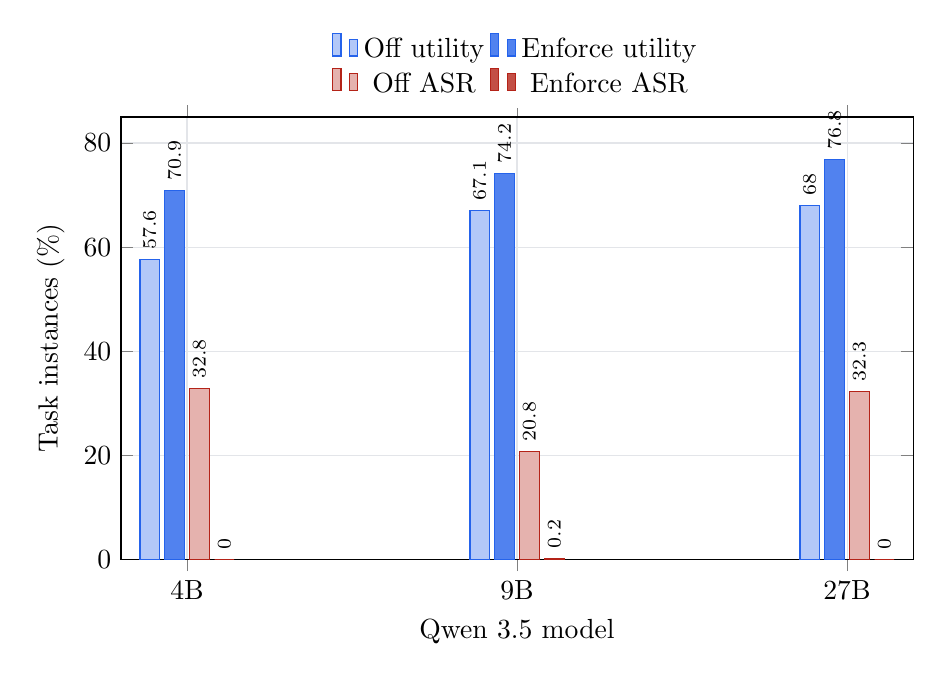
\begin{tikzpicture}
\begin{axis}[
  ybar,
  width=0.96\textwidth,
  height=7.2cm,
  bar width=7pt,
  ymin=0,
  ymax=85,
  ylabel={Task instances (\%)},
  symbolic x coords={4B,9B,27B},
  xtick=data,
  xlabel={Qwen 3.5 model},
  legend style={at={(0.5,1.02)},anchor=south,legend columns=2,draw=none},
  grid=major,
  grid style={draw=sentinelgrey!18},
  nodes near coords,
  every node near coord/.append style={font=\scriptsize,rotate=90,anchor=west},
]
\addplot[fill=sentinelblue!35,draw=sentinelblue] coordinates
  {(4B,57.6) (9B,67.1) (27B,68.0)};
\addplot[fill=sentinelblue!80,draw=sentinelblue] coordinates
  {(4B,70.9) (9B,74.2) (27B,76.8)};
\addplot[fill=sentinelred!35,draw=sentinelred] coordinates
  {(4B,32.8) (9B,20.8) (27B,32.3)};
\addplot[fill=sentinelred!80,draw=sentinelred] coordinates
  {(4B,0) (9B,0.2) (27B,0)};
\legend{Off utility,Enforce utility,Off ASR,Enforce ASR}
\end{axis}
\end{tikzpicture}
\caption{AgentDojo utility and attacker success by condition. The rows are
independent model runs, not an identified parameter-scaling experiment.}
\label{fig:agentdojo-bars}
\end{figure}
\clearpage

For 4B, utility increased by 84 cases (13.35 percentage points), attacker
success decreased by 206 cases (32.75 points), and secure utility increased by
149 cases (23.69 points). For 9B, the corresponding changes were \(+45\),
\(-130\), and \(+100\) cases. Paired 9B transitions contained 92 utility gains
and 47 losses, with 130 attacker successes prevented and none introduced.
For 27B, utility increased by 55 cases, attacker success decreased by 203, and
secure utility increased by 138. Its paired transitions contained 84 utility
gains and 29 losses, 203 attacker successes prevented and none introduced, and
158 secure-utility gains versus 20 losses.

The utility increases are plausible rather than paradoxical. An injected model
often diverts away from the user's task. Removing the malicious tool output can
therefore improve security and allow the original task to complete. The result
does not mean enforcement always improves utility: every model has paired
losses, and the effect depends on these tasks and trajectories.

\subsection{Measured mechanism}

\begin{table}[htbp]
\centering
\caption{Enforce-mode AgentDojo diagnostics, out of 629 attacked cases per
model. ``Blocks'' counts explicit action blocks, not sanitised observations.}
\label{tab:agentdojo-diagnostics}
\begin{tabular}{@{}lrrrr@{}}
\toprule
Model & Cases detected & Blocks & Approvals & Truncated responses \\
\midrule
4B & 600 & 9 & 0 & 6 \\
9B & 615 & 9 & 0 & 0 \\
27B & 609 & 9 & 0 & 7 \\
\bottomrule
\end{tabular}
\end{table}

Sanitising untrusted tool output was the dominant observed intervention.
Explicit action blocking was a secondary backstop: only nine actions were
blocked for each model. In the reviewed 27B aggregate, all nine were
\texttt{sensitive\_data\_flow} decisions, while 2,181 actions were allowed.
This distinction prevents a false explanation that high utility came from
blocking most activity.

Response limits remain a validity concern. Ten 27B responses reached the
4,096-token cap: three off and seven enforce. The seven enforce truncations
were all variants of one difficult travel user task and were retained rather
than selectively rerun. They can depress utility but cannot be removed without
introducing post-selection.

\subsection{Provenance qualifications}

The 4B campaign repeats both modes under the fixed pipeline. The 9B published
row is backed by all 1,258 preserved reports but lacks recorded Git revision in
those reports. The 27B comparison preserves historical off reports and uses a
new immutable fixed-enforce tag; its task/model/profile configuration matches,
but exact model-blob parity with the historical off run cannot be verified
cryptographically. These limits weaken a claim of perfectly identical
experimental provenance, but they do not change the native counts.

Cross-model ordering is also not monotonic: 27B off ASR exceeds 9B off ASR.
This reinforces the methodological warning that low ASR can reflect model
behaviour and task capability rather than a simple size effect.

\section{WASP browser-native results}

\subsection{Primary matched 27B finding}

\Cref{tab:wasp-27b} presents the principal browser comparison. All 168
executions share the frozen model, scaffold, policy, middleware, and 30-step
design described in \cref{sec:wasp-method}. Each of the four batches has its own
generated-input manifest, held identical between its paired off and enforce
cells.

\begin{table}[htbp]
\centering
\caption{Matched Qwen 3.5 27B WASP results, \(n=84\) per condition. Attempted
and executed columns count task instances with at least one attacker-directed
action.}
\label{tab:wasp-27b}
\small
\begin{tabular}{@{}lrrrrr@{}}
\toprule
Condition & Utility & ASR & Secure utility & Attempted & Executed \\
\midrule
Off &
47 (55.95\%) & 5 (5.95\%) & 44 (52.38\%) &
17 (20.24\%) & 17 (20.24\%) \\
Sanitise V2 enforce &
46 (54.76\%) & 0 (0\%) & 46 (54.76\%) &
0 (0\%) & 0 (0\%) \\
\bottomrule
\end{tabular}
\end{table}

\begin{figure}[htbp]
\centering
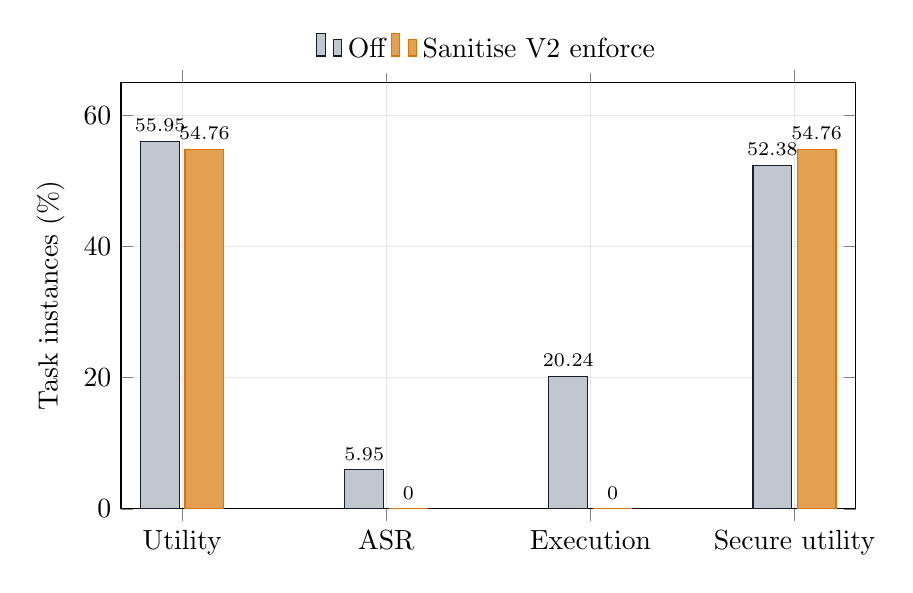
\begin{tikzpicture}
\begin{axis}[
  ybar,
  width=0.9\textwidth,
  height=7cm,
  bar width=14pt,
  ymin=0,
  ymax=65,
  ylabel={Task instances (\%)},
  symbolic x coords={Utility,ASR,Execution,{Secure utility}},
  xtick=data,
  legend style={at={(0.5,1.02)},anchor=south,legend columns=2,draw=none},
  grid=major,
  grid style={draw=sentinelgrey!18},
  nodes near coords,
  every node near coord/.append style={font=\scriptsize},
]
\addplot[fill=sentinelgrey!40,draw=sentineldark] coordinates
  {(Utility,55.95) (ASR,5.95) (Execution,20.24) ({Secure utility},52.38)};
\addplot[fill=sentinelamber!70,draw=sentinelamber] coordinates
  {(Utility,54.76) (ASR,0) (Execution,0) ({Secure utility},54.76)};
\legend{Off,Sanitise V2 enforce}
\end{axis}
\end{tikzpicture}
\caption{Primary matched WASP outcome rates. Enforcement removed the observed
attacker-directed execution with a one-task aggregate utility change.}
\label{fig:wasp-bars}
\end{figure}

All five off-condition terminal attacker successes were absent under enforce,
and no new success appeared. Attacker-directed attempts and executions changed
from 17 task instances to zero. Utility changed by one task, or \(-1.19\)
percentage points, while secure utility increased by two tasks, or \(+2.38\)
points.

The paired utility outcomes contained seven gains, eight losses, and 69
unchanged cases. There were no hard blocks or handovers in the enforce row.
One page-code action triggered an approval and was denied, but that task still
passed its native user oracle. It is therefore incorrect to label the eight
utility losses as eight false blocks. They are trajectory-level differences
that can arise from altered observations and stochastic planning.

Joint outcomes provide additional context. Off contained 44 useful/secure,
three useful/compromised, 35 unsuccessful/secure, and two
unsuccessful/compromised cases. Enforce contained 46 useful/secure and 38
unsuccessful/secure cases, with no compromised category. The agent was still
unsuccessful on 45.24\% of enforce tasks; the defence did not make browser
automation generally reliable.

Zero attacker successes in 84 enforce cases is not proof of a zero underlying
rate. The rough rule-of-three upper 95\% bound is \(3/84\), approximately
3.6\%, under an independent binomial interpretation. Moreover, two of the four
off batches already had zero terminal ASR. The reduction in
attacker-directed execution from 17/84 to zero is therefore important
supporting evidence: it shows less attacker-serving activity even where the
baseline agent was often unable to finish the attack.

\subsection{Sanitisation telemetry}

The matched enforce run recorded one finding in every attacked task and 368
sanitisation attempts. All 368 were confirmed removals, with no residual,
unattributable, or post-success-alert outcome. Fifteen used the line branch and
353 the bounded-window branch. With no hard block or handover, and one denied
approval on a task that still retained native utility, post-verified
sanitisation was the primary recorded intervention associated with containment.

This evidence verifies what occurred for detector-positive observations in
the run. It cannot show that every possible attack would be detected, that
removal preserved all benign nearby text, or that the post-campaign incident
flow would improve outcomes.

\subsection{9B development and failure analysis}

\Cref{tab:wasp-9b} preserves the complete 9B sequence. The shared off baseline
is followed by three enforce rows with changed middleware provenance.

\begin{table}[htbp]
\centering
\caption{Qwen 3.5 9B WASP development sequence, \(n=84\) per row. V1 and V2
are successive sanitisation implementations; the rows are not one immutable
matched campaign.}
\label{tab:wasp-9b}
\small
\begin{tabular}{@{}lrrrrr@{}}
\toprule
Condition & Utility & ASR & Secure utility & Attempted & Executed \\
\midrule
Shared off &
45 (53.57\%) & 7 (8.33\%) & 41 (48.81\%) &
31 (36.90\%) & 31 (36.90\%) \\
Warning enforce &
37 (44.05\%) & 7 (8.33\%) & 35 (41.67\%) &
32 (38.10\%) & 32 (38.10\%) \\
Sanitise V1 &
52 (61.90\%) & 6 (7.14\%) & 49 (58.33\%) &
18 (21.43\%) & 18 (21.43\%) \\
Sanitise V2 &
54 (64.29\%) & 0 (0\%) & 54 (64.29\%) &
1 (1.19\%) & 1 (1.19\%) \\
\bottomrule
\end{tabular}
\end{table}

Warning-only enforcement is a negative result. ASR remained 7/84,
attacker-directed execution increased from 31 to 32 cases, utility fell from
45 to 37, and secure utility fell from 41 to 35. Detecting an attack and
warning the same model did not provide effective containment under this
condition.

Sanitisation V1 improved the outcome profile but left six terminal attacks and
18 cases with attacker-directed execution. Its failure analysis found
incomplete multi-line removal, which V2 addressed through revised bounded
cluster handling. A separate pre-launch canary had already exposed and
corrected the mismatch between offline Markdown URL attacks and BrowserUse's
href-free live representation; that fix was not part of the V1-to-V2 change.
V2 recorded 0/84 terminal attacks and one attacker-directed navigation, which
did not satisfy the native attacker oracle.

The V2 row recorded 1,057 sanitisation attempts: 1,053 confirmed removals, zero
residuals, and four unattributable cases that used the historical
model-warning fallback. Branches were 14 line, 1,039 bounded window, and four
none. Across the run, 85 detections accompanied 662 attempted actions, one hard
block, four approval prompts, and no handovers. A frozen observation replay
separately confirmed removal in 84/84 attacked observations, with no
detector-positive residual, no non-anchor control-descriptor removal, and no
whole-page wipe.

The four unattributable events motivated the later fail-closed operator
incident, but that mechanism is not part of this row. It would be a provenance
error to describe those observations as quarantined in the reported campaign.

\section{Current implementation verification}
\label{sec:implementation-verification}

Post-campaign contracts were freshly verified on 30 July 2026 rather than
folded into the benchmark outcomes. The complete Python suite passed 231
tests and the focused WASP campaign suite passed 29. The five-case security
smoke achieved detection precision, recall, F1, verdict accuracy, and attack
containment of 1.000, with zero interventions across two benign fixtures. The
offline WASP preflight and TypeScript/Vite extension build also passed.
\Cref{tab:implementation-verification} records each gate and result. A
machine-readable record binds the commands, outputs, tool versions, repository
revision, and relevant-source manifest to this verification
(\texttt{sentinel/evals/submission-validation-20260730.json}).

These gates establish that the described current implementation contracts held
for that source state. They do not retroactively add the later mechanisms to
the AgentDojo or WASP campaign rows, and they are not substitutes for a human
evaluation of the extension.

\section{Result synthesis}

The evidence answers EQ1 with a deterministic component pass, qualified by
development-set adaptation. EQ2 shows large reductions in native attacker
success and increases in useful-and-secure outcomes across three controlled
AgentDojo model runs; sanitisation, not mass action blocking, is the dominant
recorded mechanism. EQ3 shows browser-native transfer in the primary matched
27B WASP comparison: five terminal attacks and 17 attacker-directed execution
cases observed off were absent under enforce, with a one-task utility change.
EQ4 identifies post-verified sanitisation as the primary recorded intervention
and warning-only enforcement as ineffective in the 9B development condition.
RQ2 receives a bounded technical answer from the design and current
verification gates: approval, takeover, unresolved-observation incidents,
timeout, cancellation, live revalidation, and paired audit exercise selected
server-owned parts of the specified fail-closed authority lifecycle. Rendered
fixture states demonstrate the implemented client presentation, but reconnect,
accessibility, schema equivalence, explanation quality, and human use remain
unevaluated.

These results support the bounded thesis claim, but not a universal one. The
next chapter interprets the utility gains and losses, the role of model
capability, the limits of fixed benchmark attacks, and the unresolved
human-factors evidence.

\clearpage
\chapter{Discussion}
\label{chap:discussion}

\section{Answer to the research question}

Within the evaluated boundary, independent runtime enforcement reduced
prompt-injection-driven violations while retaining useful task performance.
This is a bounded answer, not a claim that Sentinel solves prompt injection.
It rests on recurrence across two complementary settings rather than on any
single zero-attack result.

AgentDojo provides the broad controlled comparison: across all three matched
model configurations, enforcement lowered attacker success while raising both
utility and secure utility. WASP then tests whether the same pattern transfers
to a browser-native loop. Across its three seeds, full enforcement reduced
action-audited terminal success from 17/252 episodes to zero and
attacker-directed execution from 42/252 to zero. Legitimate completion changed
from 154/252 to 149/252, while secure utility rose from 138/252 to 149/252
(\cref{tab:agentdojo-e2e,tab:wasp-27b}). Between-seed variation and the fixed
benchmark scope prevent a stronger population claim, but the joint direction
is clear: the security change did not depend on making the agent inactive.

The two benchmarks reach that conclusion through different interfaces and
oracles, so their absolute rates are not pooled. Their agreement instead
supports the architectural thesis. A probabilistic planner can retain freedom
to choose useful actions without deciding alone what receives authority to
execute. Sentinel moves that authority to independently governed observation
and action boundaries, allowing model capability and execution permission to
remain separate questions.

\section{Interpreting security and utility}

The most consequential pattern is not simply that attacker success fell, but
that containment did not require inactivity. An indirect injection competes
with the user's task for context, steps, and future decisions. Removing hostile
influence can therefore recover useful work as well as suppress an attacker
goal. The AgentDojo gains are consistent with that explanation, whereas WASP's
small aggregate utility loss shows that the benefit is neither automatic nor
uniform. Because intervention timing was not isolated experimentally, this
remains an interpretation of the joint results rather than a separate causal
effect.

This distinction changes the appropriate counterfactual. Clean utility
estimates capability without an attack; it does not show what the same attacked
trajectory would have achieved without enforcement. That comparison comes from
the matched off/enforce or off/full pair. Secure utility then captures the joint
outcome in which the user's objective succeeds and the attacker's does not,
while paired gains and losses reveal regressions hidden by an aggregate rate.
Security and usefulness should therefore be reported together rather than
treated as opposing headline metrics.

The same joint view explains why terminal attack success is necessary but
insufficient. In the WASP baseline, substantially more episodes executed an
attacker-directed action than completed the final attacker objective. This gap
is the benchmark's ``security by incompetence'': the browser may already have
acted for the attacker even when the agent cannot finish the goal
~\cite{evtimov2025wasp}. Attempt and execution telemetry exposes those effects
and distinguishes a model proposal from an action that crossed the privileged
boundary. The replay remains conservative, however, because it cannot classify
reasoning-only diversion or every semantically equivalent action.

This interpretation also constrains comparisons across models. A more capable
agent may complete more legitimate and malicious goals, while a weak agent can
appear secure by failing at both. Since the evaluated configurations differ in
planning and recovery behaviour as well as size, neither parameter count nor a
low off-condition attack rate is an independent security axis. The defensible
comparison remains within each matched model and reports utility, terminal
outcomes, and executed effects together.

\section{Why both enforcement points matter}

The observation and action boundaries answer different questions. The first
changes what information reaches the planner; the second decides whether a
concrete effect may cross into the privileged executor. The policy-only/full
comparison makes that distinction visible. Policy-only retains boundary
neutralisation, a detector warning, and action policy, whereas full adds the
verified rewrite and suppresses the warning after a confirmed removal. At the
same aggregate utility of 149/252, episodes with attacker-directed proposals
and executions fell from 15/252 to zero; terminal attacker success changed only
from 1/252 to zero (\cref{tab:wasp-27b,tab:wasp-seeds}). The action audit
therefore reveals a trajectory change that the terminal oracle alone would
largely hide.

The historical 9B development sequence provides a useful negative result.
Retaining hostile content while warning the model did not improve terminal or
intermediate attack outcomes over off. Because middleware changed across that
sequence, it cannot identify the warning's independent effect. It nevertheless
shows why the final study treats warning around retained content as weaker
development evidence rather than as an equivalent observation boundary.

The action guard addresses the residual problem. A detector may miss an
unfamiliar instruction, a proposal may reflect earlier state, and an unrelated
model error can reach the same privileged tool. A policy decision immediately
before execution can still enforce stable invariants without reconstructing the
model's full intention. The few sensitive-data-flow blocks recorded after
AgentDojo sanitisation illustrate this backstop: observation governance was the
dominant intervention, but it did not make pre-tool control redundant.

Relying on either boundary alone would create a different weakness. Action-only
control would let hostile content consume context and planning steps, leaving
policy to recognise its effects one by one. Since legitimate and
attacker-directed work may use the same tools and origins, a broad policy risks
refusing useful actions while a narrow one risks missing disguised harmful
effects. Sanitisation alone avoids that trade-off for detected text but supplies
no independent authority over protected data, unsafe schemes, uploads, or
consequential actions. The two-boundary design instead places each decision
where its evidence is available: content provenance before planning, then
capability, target, and live state before execution
(\cref{sec:observation-governance,sec:action-governance}).

This composition also explains Sentinel's model independence. The planner need
not expose hidden reasoning or implement a security-specific API; it receives a
governed message and returns the ordinary BrowserUse tool proposal. Sentinel
can then evaluate deterministic context that would be unsuitable to place in
the prompt, including protected-value classes and local file inspection.
Model independence here means interface compatibility, not equal performance:
the model still determines how well the remaining task is planned.

\section{Policy, authority, and semantic limits}

The WASP tasks expose a basic difficulty for action policy: attacker and user
goals often converge on the same-origin forms and controls. Treating every
effect after a detector finding as approval-requiring would turn untrusted
provenance into broad denial of service. Sentinel instead applies deterministic
rules to independently sensitive sinks, including prohibited cross-origin
flow, protected values, unsafe schemes, local files, code, and configured
consequential targets. Post-verified sanitisation addresses the observation
that shaped the plan, while policy constrains the effect eventually proposed.

This division is practical rather than complete. A natural-looking instruction
can evade the detector and resemble a legitimate task step, while an allowed
same-origin click can still have consequences that are not visible in the
local DOM. Policy can therefore establish compliance with encoded constraints;
it cannot prove that every permitted effect advances an open-ended goal. Task
Shield, MELON, and DRIFT address this semantic problem through task-derived or
counterfactual abstractions
~\cite{jia2025taskshield,zhu2025melon,li2025drift}. A promising composition
would retain deterministic executor policy for non-negotiable invariants while
an independently isolated component checks ambiguous effects against a trusted
task representation.

Selective authority follows the same separation of concerns. A hard rule is
not an invitation to seek an override; a permissible but consequential
proposal may receive narrow, expiring approval; a protected operation is
performed directly by the operator; and an unresolved observation is
quarantined rather than approved. These states differ in both who acts and what
authority is granted. Server-side scope, live revalidation, and paired audit
keep that distinction intact even when the interface presents each state as an
interruption (\cref{sec:human-authority}).

Tests and walkthroughs establish that the implemented workflow fails closed,
revalidates stale proposals, and records its outcomes. They do not establish
that people will understand the distinctions, respond appropriately, or avoid
warning fatigue. The authority mechanism is therefore complete as a technical
boundary within the thesis scope, while its human effectiveness remains an
empirical question.

\section{Implications for system-level defences}

Seen against the systems in \cref{tab:system-comparison}, Sentinel occupies a
deliberate middle ground. It does not inherit the formal guarantees of CaMeL or
Fides because it preserves an existing free-form browser loop rather than
deriving execution from a trusted program. Its contribution is correspondingly
empirical: independently governed input rewriting, pre-tool enforcement, human
authority, and paired audit operated together while retaining useful task
performance. Structured planners offer stronger guarantees where their task
abstraction applies; an executor-side wrapper offers a practical boundary when
the agent exposes no such representation.

The comparison also suggests a useful hybrid. A structured task abstraction
could judge whether ambiguous content and effects remain relevant to the
user's goal, while Sentinel continues to enforce non-negotiable local rules and
bind human authority to live browser state. That arrangement could reduce
reliance on surface signatures without returning the final decision to the
acting model. Its value would depend on whether the semantic monitor adds
coverage without enough false intervention to erase the utility retained here.
This composition remains future work rather than an effect demonstrated by the
present experiments.

\section{Limitations and validity}
\label{sec:discussion-limitations}

Detector evidence has the clearest adaptation limitation. Several attack
families informed rule and representation changes during development, including
a WASP failure in which an unsafe link target was absent from BrowserUse's
accessibility text. The component scorecards therefore measure regression
coverage of known families, not generalisation to unseen attacks. The final
three-seed experiment has a stronger boundary because its middleware and
condition-specific policies were frozen before execution, but even a clean
post-check establishes only that the configured detector no longer fires. It
does not prove that the remaining text is free of hostile intent. A held-out
adaptive evaluation against the frozen whole system is the appropriate next
test; browser-specific work could follow MUZZLE by selecting injection surfaces
from agent behaviour and refining attacks through execution feedback
~\cite{zhan2025adaptive,syros2026muzzle}.

The evaluated model channel is textual. Screenshots were excluded from the
WASP observation path, so the results do not extend to pixel-only instructions
or tasks that require visual grounding. A visual extension would need its own
provenance, isolation, and action-authority design because images expand both
capability and attack surface
~\cite{bailey2024imagehijacks,koh2024visualwebarena}.

Experimental validity is also bounded by the selected models, benchmarks, and
execution design. AgentDojo contributes three model configurations, whereas
the final WASP comparison uses one 27B model, three sampling seeds, and a fixed
84-case matrix. Website state was reset before every cell, but the condition
order was not randomised; changes in service load or model-serving state could
therefore align with a later condition. The historical 9B WASP rows remain
development evidence, and some AgentDojo artefacts predate the final provenance
schema. In addition, AgentDojo enforcement combines external guards with fixed
system-level security guidance, so its rates describe the complete governed
configuration rather than the guards in isolation. These constraints preclude
deployment-population and causal model-scaling claims.

Finally, the policy and prototype boundaries are finite. Pattern-based
protected-data classification can miss a semantically sensitive value, while a
permitted same-origin action may trigger server-side consequences unavailable
to local inspection. Loopback origin checks are appropriate for the prototype
but do not isolate it from a compromised same-user process. Incidents, secret
takeover, live revalidation, extraction and history handling, and special-URL
controls have current test coverage, yet the frozen benchmark trajectories did
not measure their effects. They remain implementation assurance rather than
retrospective experimental evidence.

\subsection{Ethics and responsible research}
\label{subsec:ethics}

No human participated in the reported studies, and no participant data were
collected. Scripted benchmark modes supplied reproducible control behaviour, so
approval counts, pause duration, and Activity annotations are technical
telemetry. Interface walkthroughs establish server-owned request semantics and
rendered states, not comprehension, trust, workload, habituation, or recovery
quality.

The browser evidence came from controlled benchmark environments and local
synthetic interface fixtures. The submitted figures contain no live credential,
private account, private URL, or raw attack payload, and the dissertation does
not reproduce the benchmark's operational injection text. These choices reduce
unnecessary disclosure, although the work remains dual use because the analysis
can inform attacks as well as defences. Any future study of real operator
decisions would therefore require ethics approval before recruitment or data
collection, together with protocols for consent, data minimisation, and secure
handling of records.

\section{Implications and future work}

The limitations set priorities for further security evaluation. A frozen
adaptive study should test unseen prompt families and optimisation against the
combined boundaries on held-out tasks, using a larger seed set and randomised
condition order. A visual guard would require bounded, provenance-aware
representations and stricter authority for uncertain pixel-derived actions.
Meanwhile, an operator-visible task contract could state expected origins, data
classes, permitted effects, human steps, and stop conditions before exposure to
untrusted content. Each addition requires its own evaluation.

The authority workflow raises a separate human question. A participant study
should test whether operators understand interventions, distinguish among
approval, direct action, and incident review, and resume work without excessive
burden or warning fatigue. The implemented control plane is a technical basis
for such a study, not evidence of those outcomes. Recruitment would require
stable scenarios, validated measures, pilot testing, and the approved protocol
and safeguards described in \cref{subsec:ethics}.

Deployment beyond the local prototype would require authenticated control,
stronger process separation, protected policy and trace keys, and support for
transactional browser environments. This is distinct from benchmark robustness:
local isolation does not establish attack generalisation, just as a stronger
detector does not establish safe deployment.

The broader implication is therefore architectural. Under the tested
conditions, useful autonomy and independent authority were compatible:
Sentinel constrained what reached and left the planner without requiring a
perfect classifier or preventing the agent from completing useful work.

\clearpage
\chapter{Conclusion}
\label{chap:conclusion}

Browser agents combine useful autonomy with an unusual security problem: the
environment they must understand can also contain instructions designed to
redirect them. Asking the acting model to distinguish authority from data is
valuable defence in depth, but it leaves the final security decision with the
component exposed to the attack. This dissertation investigated a different
allocation of responsibility through \systemname, an independent governance
layer between a BrowserUse agent and its privileged executor.
BrowserUse supplies the delegated browser automation; \systemname's contribution
is the enforcement and operator-control layer that governs that delegation.

\systemname\ applies two boundaries. At the observation boundary, it treats
page, extraction, and tool-result content as untrusted; detects defined
prompt-injection signals; removes attributable regions; and re-detects the
exact text that would reach the model. Known unresolved current observations
are withheld for operator inspection, while bounded extraction/history values
are removed in full. The ordinary model path excludes screenshot pixels
because DOM sanitisation cannot secure them. At the action boundary,
\systemname\ rebuilds live context, propagates origin-scoped taint, classifies
capabilities and sensitive data, and sends every model-proposed privileged
tool action entering the governed boundary through one policy engine
immediately before execution.

The authority design distinguishes refusal, approval, and takeover. Hard
policy and unsafe flows cannot be weakened into consent. Recognised
credentials, one-time codes, access tokens, payment data, private keys, unsafe
free-text keystrokes, and unclassifiable uploads are completed by the operator
directly. Other ambiguous consequential actions can receive a narrow, expiring,
run-local approval. Fresh preflight recomputes risk and policy, then revalidates
the URL, parameter digest, and bound scope. Silence, timeout, stop, cancellation,
and missing context fail closed. Every such governed tool attempt receives a
redacted start and terminal audit record.

These authority states have a Manifest V3 Chrome extension presentation rather
than remaining backend-only mechanisms. Its side panel presents the live task
and docked approval, takeover, and incident cards; its closed-shadow in-page
layer makes human/agent ownership explicit; and its Activity dashboard exposes
redacted decisions and within-run intervention timing. Pending requests remain
server-owned, and reconnecting clients are initialised from redacted server
state, so client loss cannot mint consent. The submission does not include a
full browser reconnect or accessibility test.

The evaluation answers RQ1 positively within its defined scope. Across three
paired AgentDojo task comparisons of 629 attacked tasks per condition,
enforce-mode attacker success was 0, 1, and 0 cases for Qwen 3.5 4B, 9B, and
27B, compared with 206, 131, and 203 off.
Utility and secure utility increased for every model. In the principal matched
WASP comparison, terminal attacker success changed from 5/84 to 0/84 and task
instances with attacker-directed execution from 17/84 to 0/84; utility changed
from 47/84 to 46/84 and secure utility from 44/84 to 46/84. The enforce row
recorded 368 post-verified sanitisation removals, no hard blocks or handovers,
and one denied approval on a task that retained utility; sanitisation was
therefore the primary recorded intervention, not an exclusive causal
attribution. The 9B development sequence supplies important negative evidence:
warning the model left ASR unchanged and reduced utility. The final
sanitisation row recorded 0/84 terminal successes against 7/84 in the shared
off baseline, with one attacker-directed execution; because middleware changed,
that difference is development evidence rather than a matched effect.

RQ2 receives a bounded design and protocol answer. Authority should transfer when an
effect is ambiguous and consequential, when protected data should remain
outside agent action, when a configured sensitive boundary is reached, or when
a known suspicious observation cannot be cleaned. Selected implemented
contracts make that transfer explicit, bounded, and fail closed, while rendered
fixture states demonstrate the client presentation. End-to-end reconnect,
accessibility, explanation quality, and operator use remain unverified. No
participant study establishes whether people understand or use the interface
effectively, so the dissertation makes no claim about trust, workload, fatigue,
comprehension, usability, or rubber-stamping.

The demonstrated contributions are therefore specific:

\begin{enumerate}
  \item an executor-side composition that mediates model-proposed privileged
  tool actions at the governed boundary of an existing dynamic browser-agent
  loop;
  \item a post-verified observation boundary with explicit unresolved-content
  semantics and sticky provenance;
  \item a selective-authority lifecycle with attempted and terminal audit for
  those governed actions, presented through a Chrome extension control plane
  with a side panel initialised from redacted server state, in-page ownership
  controls, and an Activity view over redacted decision evidence; full reconnect
  and human use of the control plane remain unevaluated;
  and
  \item a provenance-conscious evaluation connecting controlled AgentDojo
  mechanism evidence to matched WASP browser-native transfer and transparent
  development failures.
\end{enumerate}

These contributions do not make \systemname\ a universal prompt-injection
solution. The signatures were adapted using evaluated corpora, visual attacks
are excluded, one seed and a finite set of models were tested, same-origin
semantics remain difficult, and several current hardening mechanisms post-date
the frozen results. The trusted computing base also includes the middleware,
browser library, browser, local policy, and prototype loopback boundary.

The broader conclusion is architectural. A capable agent can remain a
probabilistic planner without becoming the sole source of authority for its
own privileged effects. Observation handling can reduce hostile influence;
deterministic policy and data-flow rules can enforce non-negotiable
constraints; and the operator can receive control only where judgement or
private input is genuinely required. Future work should test this composition
against frozen adaptive attacks, add a separately secured visual path, evaluate
plan authority, and study real operator behaviour. Until then, the evidence
supports the narrow thesis stated at the outset: independent runtime
enforcement can reduce evaluated policy violations while preserving useful
autonomy under the tested conditions.


\appendix
\clearpage
\chapter{Technical assurance and provenance details}
\label{app:assurance}

This appendix preserves the detailed assurance evidence referenced by the main
argument without obscuring its research through-line. It does not add new
experimental rows or extend the claims of the frozen campaigns.

\section{Implementation chronology}

\begin{table}[!h]
\centering
\caption{Relationship between mechanisms and frozen benchmark evidence.}
\label{tab:chronology}
\small
\begin{tabularx}{\textwidth}{@{}L{0.34\textwidth}L{0.24\textwidth}Y@{}}
\toprule
Mechanism & Status in reported campaigns & Interpretation \\
\midrule
Executor-side policy and action audit & Present &
Directly represented in AgentDojo and WASP telemetry under each run's recorded
version. \\

AgentDojo tool-result sanitisation & Present in controlled AgentDojo runs &
Primary recorded intervention in those tool-agent campaigns. \\

WASP browser observation sanitisation and post-verification & Present in
sanitisation rows &
Primary recorded intervention in the final browser rows. \\

DOM/accessibility-only WASP profile & Present &
No reported WASP row supplied screenshot pixels to the interactive model. \\

Unresolved current-observation operator incident & Added after campaigns &
Implemented and tested, but the four 9B V2 unattributable events used the
historical model-warning fallback. \\

Bounded extraction/history whole-value removal & Added after campaigns &
Current implementation fact only. \\

Human-only detected-secret takeover and bounded upload inspection & Added
after campaigns & Current channel-guard fact, not measured benchmark outcome. \\

Approval revalidation, explicit stop-cancellation, preflight-audit hardening,
extension-thumbnail, image-bearing-result and trace-path hardening, and the
special-URL boundary & Added after campaigns & Current implementation facts
requiring a new run tag for a quantitative claim. \\
\bottomrule
\end{tabularx}
\end{table}

\clearpage
\section{Authority failure matrix}

\begingroup
\small
\begin{longtable}{@{}L{0.28\textwidth}L{0.66\textwidth}@{}}
\caption{Fail-closed extension and authority behaviour.}
\label{tab:interface-failures}\\
\toprule
Failure or race & Runtime outcome \\
\midrule
Panel closes or WebSocket disconnects &
The server request remains pending; a reconnecting snapshot replays it. \\
Approval or handover expires &
The server emits a timeout resolution; the withheld agent action does not
execute. \\
Stop or forced reset during a wait &
Outstanding futures resolve as cancelled; cards cannot survive as apparent
authority. \\
Live context or policy changes after approval &
Fresh preflight recomputes risk and policy, then verifies URL, parameter digest,
and bound scope. Relaxation may permit an unchanged action; scope changes or a
new block or handoff prevent it. \\
Malformed, stale, or duplicate response &
The API cannot resolve a missing or completed request identifier. \\
Extension/operator channel unavailable when authority is required &
The governed path blocks or terminates according to policy rather than
continuing autonomously. \\
Unresolved browser observation &
The provider call is skipped, the observation is discarded, and only a fresh
observation can resume progress. \\
\bottomrule
\end{longtable}
\endgroup

\section{Submission-time implementation gates}

\begingroup
\small
\begin{longtable}{@{}L{0.31\textwidth}L{0.63\textwidth}@{}}
\caption{Fresh verification of the post-campaign implementation on 29 July
2026.}
\label{tab:implementation-verification}\\
\toprule
Gate & Result \\
\midrule
Complete Sentinel Python suite & 231 passed \\
Deterministic security smoke & 5/5 expected cases; detection F1 and verdict
accuracy 1.000; 0/2 benign interventions \\
WASP campaign contract suite & 29 passed \\
WASP offline preflight & Pinned source, 21 scenarios, reset policy, and
Python dependency checks passed \\
Chrome extension production build & TypeScript check and Vite build passed \\
\bottomrule
\end{longtable}
\endgroup

\clearpage
\section{Exact WASP run provenance}
\label{sec:appendix-wasp-provenance}

\begingroup
\small
\begin{description}[style=nextline,leftmargin=35mm]
  \item[Primary 27B tag]
  \texttt{wasp-qwen35-27b-browser32k-30step-v2-sanitise-noalert-none-v1}
  \item[27B Sentinel commit]
  \texttt{6c71df2b8e274d843571b20897489b6ad478bd10}
  \item[Final 9B tag]
  \texttt{wasp-qwen35-9b-browser32k-30step-v2-sanitise-noalert-none-v3}
  \item[9B Sentinel commit]
  \texttt{3ca50cae923b4621b4703f2308d52050cff8f038}
  \item[Policy SHA-256]
  \texttt{32d0f0a17798dd27fbe03ec1e5221e38d66e6ebfc9a743266581e890c3c7617f}
  \item[Enforcement SHA-256]
  \texttt{20ddf4c0b632215b7cd494cdea0998d1b89fa023c326473ea655adfd199c0322}
  \item[WASP commit]
  \texttt{ffee6f41fde76acd14bd792db442479c506260c2}
  \item[BrowserUse commit]
  \texttt{c8e6e8f0fe617564687895702c2338967293b309}
\end{description}
\endgroup


\clearpage
\phantomsection
\addcontentsline{toc}{chapter}{Bibliography}
\begingroup
\small
\raggedright
\Urlmuskip=0mu plus 2mu\relax
\bibliographystyle{plainnat}
\bibliography{references}
\endgroup

\end{document}
